\documentclass[a4paper,11pt]{article}
\usepackage[utf8]{inputenc}
\usepackage[T1]{fontenc}
\usepackage[top=1.5cm, bottom=1.5cm, left=1.5cm, right=1.5cm]{geometry}

\title{Semantically checked source code merge}
\author{Guillaume Bertholon, supervised by Yann Régis Gianas, IRIF -- Université de Paris}

\usepackage{listings-rust}
\lstset{
  language=Rust,
  breaklines=true,
  extendedchars=true,
  captionpos=b,
  style=boxed,
  escapechar=@,
  % We want to disable any syntax coloring to focus on awareness colors
  stringstyle=,
  keywordstyle=,% reserved keywords
  keywordstyle=[2],% traits
  keywordstyle=[3],% primitive types
  keywordstyle=[4],% type and value constructors
  keywordstyle=[5],% macros
}

\usepackage{tikz}
\usetikzlibrary{calc}
\usetikzlibrary{positioning}
\usetikzlibrary{shapes.geometric}
\tikzstyle{varnode} = [draw, circle, text height=1.5ex, text depth=.25ex, align=center]
\tikzstyle{mvnode} = [draw, regular polygon, regular polygon sides=3, text height=1.5ex, text depth=.25ex, align=center, inner sep=2]
\tikzstyle{changenode} = [draw, rectangle, scale=0.8]
\tikzstyle{condnode} = [draw, diamond]
\tikzstyle{conflict} = [red, fill=red!10]
\tikzstyle{colorA} = [fill=blue!30]
\tikzstyle{colorB} = [fill=orange!40]
\tikzstyle{colorDel} = [fill=red!20]
\tikzstyle{colorIns} = [fill=olive!20]

\usepackage{bussproofs}
\usepackage{amsmath}
\usepackage{soul}
\usepackage{amssymb}
\newcommand\typsep{\mathrel{|}}
\newcommand\merge{\mathbin{\Join}}
\newcommand\mathst[1]{\text{\st{$#1$}}}
\newcommand\mathul[1]{\text{\ul{$#1$}}}
\newcommand\id{\square}
\newcommand\change[2]{\mathst{#1} \rightarrow \mathul{#2}}
\DeclareMathOperator\InsConflict{Ins!}
\DeclareMathOperator\DelConflict{Del!}
\DeclareMathOperator\OrdConflict{Ord!}
\DeclareMathOperator\MvConflict{Mv!}
\DeclareMathOperator\dom{dom}
\newcommand\rtstate[3]{\langle #1, #2, #3\rangle}
\newcommand\vrtstate[3]{\left\langle\begin{matrix}#1,\\#2,\\#3\end{matrix}\right\rangle}
\allowdisplaybreaks

\usepackage{hyperref}
\hypersetup{hidelinks}

\newcommand\yrg[1]{{\color{red}{(\textbf{YRG:} #1)}}}
\newcommand\gb[1]{{\color{blue}{(\textbf{GB:} #1)}}}
\newcommand\todo[1]{{\color{teal}(\textbf{TODO:} #1)}}

\usepackage[title]{appendix}
\usepackage[section]{placeins}

\begin{document}

\maketitle

\noindent {\color{red}This report uses colors for examples. Therefore it will be hard to read if printed in grayscale.}

\subsection*{The general context}

% \todo{What is it about ? Where does it come from ? What is the state of the art in this area ?}

In software engineering, people rarely work alone on large
projects. Therefore, quite often they want to merge their work with
what has been done by others in the meantime.
%
To automate these fusions, and keep track of the changes, developers
use dedicated tools named \textit{version control systems}. The most
used one nowadays is Git \cite{git}.

In the terminology of software evolution, a \textit{commit} is an
atomic action of changing several source code files that makes sense
by itself (whatever this may mean for the programmer). Typical commits
include refactorings, bug fixes or the introduction of new features.

Programmers make commits simultaneously, being unaware of what other
programmers may have done at the same time. However, the final product
is a fusion of what they all did. This space of unawareness can lead
to subtle bugs, that cannot be seen if people only review changes and
not the final code\footnote{Modern coding techniques involve
  continuous integration testing \cite{fowler2006continuous} to
  mitigate that, but tests cases are not perfect, so we want to expose
  another approach.}.

\subsection*{The research problem}

% \todo{What is the question that you studied ?
% Why is it important, what are the applications/consequences ?
% Is it a new problem ?
% If so, why are you the first researcher in the universe who consider it ?
% If not, why did you think that you could bring an original contribution ?}

The current tools to merge concurrent changes are purely textual and
line-oriented: as long as two modifications modify distinct lines of
code, a system like Git accepts to merge them
automatically. Unfortunately, even if two modifications are physically
separated, they may interact, especially when one modification breaks
the assumptions on top of which the other has been conceived.  We will
show on running examples that this can be a source of bugs.

Instead, we want to develop a semantically sound notion of commits
merge which detects that kind of unforeseen interactions between
concurrent modifications.

This new detection of conflicts can help programmers to make software
more robust, as they will be able to trust that a merge operation will
not silently introduce unwanted behaviors.

The study of the semantics of differences between two programs is not
new \cite{benton2004simple}, but some work has been done recently to
introduce the notion of correlation oracle \cite{girka2017verifiable}
to represent a rich set of verifiable relations between reduction
traces. However, to my knowledge, relational analysis has never been
applied to the specific problem of giving semantic guarantees for the
merging operation in version control systems.

\subsection*{Your contribution}

% \todo{What is your solution to the question described in the last paragraph ?
% Be careful, do \emph{not} give technical details, only rough ideas !
% Pay a special attention to the description  of the \emph{scientific} approach.}

Resolving the problem by a purely semantic merging was considered hard
for reasons explained in Section~\ref{sec:overview}. Therefore, we
tried to split the problem, and solve each step independently. This
internship proposes a merging tool based on two distinct main
components, which also are the two main contributions: (i) an
algorithm which implements a principled notion of syntactic merge at
the level of syntax trees (Section~\ref{sec:syntactic-merge}) ; (ii) a
semantic notion of unambiguous merge at the level of execution traces
(Section~\ref{sec:semantic-merge}).

\subsection*{Arguments supporting its validity}

% \todo{What is the evidence that your solution is a good solution ?
% Experiments ? Proofs ?
% Comment the robustness of your solution: how does it rely/depend on the working assumptions ?}

Our syntactic merge algorithm works on any language that can be parsed
into a syntax tree, provides good fusion in presence of refactorings,
and never favors a commit over another. As we shall discuss in
Section~\ref{sec:related-work}, it improves on existing approaches of
syntactic merge. Moreover, we were able to provide a working
implementation that behaves as expected on tested cases, and provides
provenance color annotations for the next step.
Section~\ref{sec:merge_properties} shows additional good properties
that should derive from the exposed design principles but whose formal
proof is left for future work.

For semantic guarantees, we offer a practical, expressive, and
original notion of unambiguous merge, and derive a runtime analysis
for checking it. We ensure that whenever a commit break invariants on
which another commit relied on, the user will be forced to take
action. As we do not have much information about the intents behind
source code changes, this can generate many conflicts, but always
enough. We then provide a simple way of patching the merged program to
resolve these conflicts.  Unfortunately, this part is specific to a
particular programming language, but we demonstrate how it should work
for languages that provide both functional and imperative features,
to make it easily adaptable to a large set of programming languages.

\subsection*{Summary and future work}

% \todo{What is next ? In which respect is your approach general ?
% What did your contribution bring to the area ?
% What should be done now ?
% What is the good \emph{next} question ?}

At the end of the internship, we have developed a new merging process
that produces a non-surprising~\yrg{predictable?} syntactic fusion of
changes and then forces programmers to review all potential bad
interactions between concurrent commits. The syntactic merging part is
supported by an implementation.

This achievement could become a starting point for further work that
also tries to avoid unintended behaviors introduced during code
merging.

However, our approach still need improvements to provide more
theoretical guarantees, and be usable in the real world.

For the syntactic merging algorithm a lot of properties remain to be
proven. The given algorithm does not come yet with a proof that it
respect the intended specifications; specifications that might
themselves need some improvements.

Moreover, the average user's feelings about the produced merged
differences have not been tested thoroughly, and better merging
paradigms can still be found.

On the semantic check part, what we give is only a theoretical
foundation because runtime trace analysis cannot reasonably be run on
all possible inputs to give full program guarantees. However, our work
opens the way for a static analysis that checks our runtime properties
to remove this flaw, and finally provides a running implementation of
the system.

For the conflict and ambiguity resolution system, the tactics given in
this paper are rather weak and low-level, pushing all the checking
burden on the programmer. More automated strategies could be added to
ease the workflow and maybe even remove most false-positive
ambiguities.

\section{Overview}
\label{sec:overview}

This section shows on a running example how a purely textual merge of
modifications can introduce bugs. Then, we will explain the
architecture of our tool which is based on two main components and
illustrate how it captures these bugs as semantic conflicts (called
ambiguities) between the commits.

\subsection{Problems with textual line-based approach}
Merging changes while preserving the original intent of the
developers is non trivial. The usual method implemented in version
control systems takes a textual line-based approach. We typically have
three files: a common base and two modified versions. We first compare
the base against each modification to create a line-to-line alignment
minimizing changes. Then we try to merge these changes. If the same
line in the base is modified in two distinct ways, we declare a
conflict, else we apply the single change. This method works on any
kind of textual data, but is mainly used for code. However, it fails
to capture any semantic, and this can cause undesired conflicts or,
worse, this approach can create bugs.

\noindent
\begin{minipage}{\textwidth}
\begin{minipage}{.32\textwidth}
\begin{lstlisting}[rulecolor=\color{blue!20}]
// Blue commit
fn f(c: bool) -> i32 {
    let x = answer();
    let y = if c {
        2
    } else {
        x * x
    };
    x / y
}

fn answer() -> i32 {
    let a = 2;
    let b = 40;
    a + b
}
\end{lstlisting}
\end{minipage}\hfill
\begin{minipage}{.32\textwidth}
\begin{lstlisting}
// Original
fn f(c: bool) -> i32 {
    let a = 2;
    let b = 40;
    let x = a + b;

    let y = if c {
        2
    } else {
        x
    };
    x * y
}
\end{lstlisting}
\end{minipage}\hfill
\begin{minipage}{.32\textwidth}
\begin{lstlisting}[rulecolor=\color{orange!30}]
// Orange commit
fn f(c: bool) -> i32 {
    let a = 4;
    let b = 41;
    let x = a + b;

    let y = if c {
        0
    } else {
        x
    };
    x * y
}
\end{lstlisting}
\end{minipage}
\vspace{-.4cm}
\begin{lstlisting}[label=lst:overview_commits, caption={A source code and two concurrent commits on it}]
\end{lstlisting}
\end{minipage}

\begin{lstlisting}[label=lst:overview_git_merge, caption={Output of git merge with the two commits above}]
 fn f(c: bool) -> i32 {
<<<<<<< Blue commit
    @\color{blue}let x = answer();@
=======
    @\color{orange}let a = 4;@
    @\color{orange}let b = 41;@
    let x = a + b;

>>>>>>> Orange commit
    let y = if c {
        @\color{orange}0@
    } else {
        @\color{blue}x * x@
    };
    @\color{blue}x / y@
}

@\color{blue}fn answer() -> i32 \{@
    @\color{blue}let a = 2;@
    @\color{blue}let b = 40;@
    @\color{blue}a + b@
@\color{blue}\}@
\end{lstlisting}

On the example above, we show two problems with the line-based
approach. First, the refactoring in blue does not compose with value
changes in orange. This creates the conflict shown between Lines~$2$
and~$9$. Secondly, the fusion of both codes creates a runtime bug on
Line~$15$: the implicit assumption that $y$ is non null is broken by
orange on Line~$11$, but this is silently accepted. We say that when
$c$ is true, $x / y$ is an ambiguous expression because its result
only comes from the fusion itself. Moreover, we can notice that the
absence of conflict on Lines~$10$~to~$14$ is only due to the code
formatting style, if the same if-expression was written on a single
line, there would be a conflict there. Globally, the example shows
that by not knowing anything about how a program is executed, textual
merge creates conflicts both too often to accept refactorings and not
often enough to avoid introducing bugs.

\subsection{A new merging algorithm}
In this paper, we try to fix the problems exposed above with a new
merging process.  This section reuses the previous example
(Listing~\ref{lst:overview_commits}) to expose the key ideas, the full
description being given later.

\paragraph{Two phase approach}
In order to compare program semantics, the standard approach requires
to align executions (or just codes), and deduce properties on
similarities and differences. In a merge process we also need such
alignment between concurrent versions to tell how to interleave the
changes and when they interact. This alignment must therefore be given
by something, and for practical reasons, it should be automated.

In this work, I chose to try to use a syntax driven alignment of
changes. This choice should feel quite natural for programmers because
syntax is already their way of communicating the semantic of the
program. Furthermore, syntax can be used as the input of subsequent
semantic analysis to detect bad interactions.

Following this approach, we split our merge procedure into two
distinct phases. We first syntactically merge both commits. This
solves the change alignment problem but does not prevent creating bugs
when merging. These new bugs come from the fact that each commit
assumes some invariants about the program that can be broken by
another concurrent commit.

That is why we run as a second phase a semantic analysis on the merged
syntax tree to deduce which program states are ambiguous. A program
state is semantically ambiguous if it comes from a modification whose
invariants may have been broken by another modification. Initially, as
the fusion algorithm is not aware of the precise invariants, any value
that comes from none of the commits in particular but only their
combination will be considered ambiguous.  These ambiguity points,
should then be manually reviewed, and resolved.  \yrg{I think that
  this paragraph is important and could be made clearer.  You should
  try to justify a little bit more the approach and the problem it
  solves.  } \gb{J'ai réécrit une bonne partie du paragraphe pour
  essayer d'améliorer l'explication de la coupure du problème en deux
  et de l'existance de la phase de vérification sémantique.}

\paragraph{Syntactic merge}
Similarly to what line-based merge do, we first want to compute
individual differences between the common base and each of the
commits. However here, differences are not based on lines of code but
on the syntax tree itself. This means that differences are structural,
represented as syntax trees of an extension of the source
language. Indeed, in addition to normal code, differences can have
\ul{insertions}, \st{deletions}, local replacements, unchanged holes
(depicted as $\id$), or multi-source multi-target code moves (depicted
as Greek letters) to abstract away sub-trees that are irrelevant for
the commit and ease fusion later. These notions will be explained in
further detail in Section~\ref{sec:syntax_tree_def}.

To keep track of which commit introduced which modification we use
colors. Each commit is associated with a tint. If a change has a given
tint, then the corresponding commit is aware (or unaffected) by
it. The color that we call white is given to the expressions of the
source program and is considered as having all the tints at once as
their values is supposed to be known by all the committers. In the
example, left commit has blue tint, and right commit has orange
tint. We can see in their difference that they taint the code they
introduced and the modification they made.

\noindent
\begin{minipage}{\textwidth}
\begin{minipage}{.32\textwidth}
\setstcolor{blue}
\setulcolor{blue}
\newbox\boxsemicolon
\sbox\boxsemicolon{\color{blue}\texttt{;}}
\begin{lstlisting}[rulecolor=\color{blue!20}]
fn f(c: bool) -> i32 {
    @\st{$\alpha$;}@
    @\st{$\beta$;}@
    let x = @\st{$\gamma$} $\rightarrow$@
        @{\color{blue}\ul{answer()}}@;
    let y = if @$\id$@ {
        @$\id$@;
    } else {
        @\st{$\delta$} $\rightarrow$ \ul{$\delta$ {\color{blue}*} $\delta$}@
    };
    @\st{$\delta$ * $\epsilon$} $\rightarrow$ \ul{$\delta$ {\color{blue}/} $\epsilon$}@
}

@{\color{blue} \ul{fn answer() -> i32 \{}}@
    @\ul{$\alpha${\usebox\boxsemicolon}}@
    @\ul{$\beta${\usebox\boxsemicolon}}@
    @\ul{$\gamma$}@
@{\color{blue} \ul{\}}}@
\end{lstlisting}
\end{minipage}\hfill
\begin{minipage}{.32\textwidth}
\newbox\boxtwo
\sbox\boxtwo{\setulcolor{orange}\setul{-.75ex}{}\ul{\texttt{2}}}
\newbox\boxforty
\sbox\boxforty{\setulcolor{orange}\setul{-.75ex}{}\ul{\texttt{40}}}
\begin{lstlisting}
fn f(c: bool) -> i32 {
    @\setstcolor{blue}\st{let a = {\usebox\boxtwo};}@
    @\setstcolor{blue}\st{let b = {\usebox\boxforty};}@
    let x = @\setstcolor{blue}\st{a + b}@ @$\rightarrow$@
        @{\color{blue}\ul{answer()}}@;
    let y = if c {
        @\setstcolor{orange}\st{2} $\rightarrow$ {\color{orange}\ul{0}}@
    } else {
        @\setstcolor{blue}\st{x} $\rightarrow$ \setulcolor{blue}\ul{x {\color{blue}*} x}@
    };
    @\setstcolor{blue}\st{x * y} $\rightarrow$ \setulcolor{blue}\ul{x {\color{blue}/} y}@
}

@{\color{blue}\ul{fn answer() -> i32 \{}}@
    @\setulcolor{blue}\ul{let a = {\color{orange}4};}@
    @\setulcolor{blue}\ul{let b = {\color{orange}41};}@
    @\setulcolor{blue}\ul{a + b}@
@{\color{blue}\ul{\}}}@
\end{lstlisting}
\end{minipage}\hfill
\begin{minipage}{.32\textwidth}
\setstcolor{orange}
\setulcolor{orange}
\begin{lstlisting}[rulecolor=\color{orange!30}]
fn f(c: bool) -> i32 {
    let a = @\st{2} $\rightarrow$ {\color{orange}\ul{4}}@;
    let b = @\st{40} $\rightarrow$ {\color{orange}\ul{41}}@;
    @$\id$@;

    let y = if @$\id$@ {
        @\st{2} $\rightarrow$ {\color{orange}\ul{0}}@
    } else {
        @$\id$@
    };
    @$\id$@
}





@@
\end{lstlisting}
\end{minipage}\hfill
\vspace{-.4cm}
\begin{lstlisting}[label=lst:overview_diffs, caption={Left (resp. right) represent the difference between original source code and blue commit (resp. orange commit). Center is the syntactic fusion of these two differences.}]
\end{lstlisting}
\end{minipage}

After having generated individual syntactic differences, we can merge
them and remove holes by reusing the original program, producing the
code above in the middle. This process is designed such that it never
makes any arbitrary choices, and can sometimes generate conflicts when
no canonical choice exists. However, it tries whenever possible to
push the changes following moved code to ease refactoring fusions (see Lines~$15$ and~$16$). This process propagates awareness colors.

At the end of this phase, we have a merged syntax tree that, unlike line-based merge, does not conflict on refactorings based on code moves, and enforce some structure in the changes. However, we lose the ability to commit files that do not parse, and we still do not provide any guarantee about ambiguities. For this reason, we need a second phase.

\paragraph{Semantic check}
This phase runs an analysis on the colored merged program to check that there is no ambiguous program state. Ambiguity can be linked to the color black (i.e. without any tint), because it means that two modifications were affected by each other and could have broken their respective invariants.

For technical reasons that will be explained in Section~\ref{sec:colored-diff-oracle}, the analysis must run on execution interleaving of the original base program and the merged one.

In our example, the color black appears for instance on Line~$11$ when $c$ is true, because variable~$x$ gets a blue color on Line~$4$, and variable~$y$ gets an orange color on Line~$7$, therefore value on
Line~$11$ is not known by any commit. It also appears on Line~$16$
and~$17$ as orange is not aware that its code has been moved, and blue could theoretically have reordered instructions.

To finish this example, we need a user to be able to efficiently
resolve the conflicts. Here the programmer could notice that, on
Lines~$2$ to~$5$ and~$14$ to~$18$, blue has done only semantic
preserving changes and would manually replace the blue color by white
in each of these lines. Then, an ambiguity on Line~$11$ will still
remain but it could be resolved by overriding the expression in the
merged commit by a new one like for instance
\lstinline$if y == 0 { 0 } else { x / y }$.
Therefore, given this information, the two commits
can be safely merged with the guarantee that no unintended
behavior\footnote{Problems like side channel attack vectors might still be silently introduced unless we also model them into the analysis.} will be silently introduced by the fusion itself.

\section{Syntactic merge}
\label{sec:syntactic-merge}

In this section, we present two contributions: first a procedure that
takes concurrent commits and merge them together ; second, a
provenance annotation mechanism on the merged program to allow for a
subsequent semantic aware analysis of ambiguity.

From a bird-eye view, this syntactic merge first computes individual
differences from the common ancestor to each commit, and then merges
the differences trees into a single one. Finally, we can apply the
merged difference tree to the common ancestor and obtain a
syntactically valid merge candidate. This program may not be the
desired final merged code as it is not necessarily free
from conflicts, ambiguities or even compile-time errors, but it is a synthesis of all the modifications, and should be a good base for manual resolution of conflicts.

\subsection{Syntax tree difference}

\subsubsection{Definition of syntax tree differences}
\label{sec:syntax_tree_def}
As said earlier, we encode program differences as a new kind of syntax
tree that follows the constructors from the target language and add
new ones.

Basically, a difference can be viewed as two syntax trees, a deleted one, and an inserted one. Therefore the simplest valid difference from code $d$ to code $i$ is simply the change $\change{d}{i}$, removing all $d$ and inserting $i$ as a replacement.

However, to ease fusion and produce less redundant and more readable output, we change two things.
First, we merge together identical constructions between the deletion and insertion tree starting from the root.
Secondly, we elide identical sub-trees that are present in both $d$ and $i$.

\paragraph{Merging the spine}
Trying to merge together two nodes in the syntax tree is easy, we simply need to check if they use the same root constructor, recursively merge if it is the case, and stop the process otherwise.

However, this approach shows its limits in presence of sequences ({\it e.g.} sequences of functions or sequences of statements). If we consider that the sequence constructor contains its size, sequences with only one element inserted or removed will have all their common elements still written twice.
Otherwise, if we encode the sequence with Cons/Nil constructors (like OCaml's list), elements will always be inserted/removed at the end, almost always generating sub-optimal differences.
Therefore, we use sequence edit scripts \cite[§3.Alignment]{miraldo2017type} \gb{I am not refining sequence edit script themselves, the algorithm to find them however is a refinement of LCS.} instead as the output of a merge operation on two sequences.

We call ``spine'' the merged part of the difference tree. Figure~\ref{fig:spine_seq_align} gives an example of such spine.

\begin{figure}[ht]
\begin{minipage}{0.49\textwidth}
\centering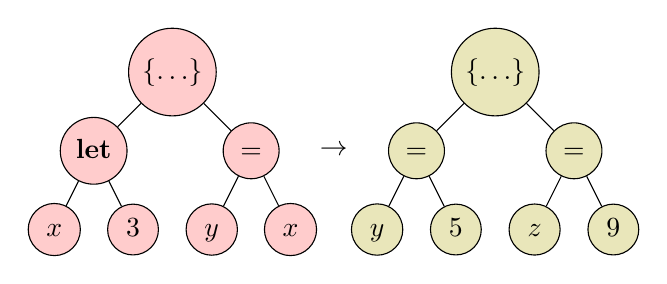
\begin{tikzpicture}
    \node[varnode, colorDel] (del_block) {$\{\ldots\}$};
    \node[varnode, colorDel] (del_stmt1) at ($(del_block)+(-1,-1)$) {$\textbf{let}$};
    \node[varnode, colorDel] (del_stmt2) at ($(del_block)+(1,-1)$) {$=$};
    \node[varnode, colorDel] (del_x) at ($(del_stmt1)+(-0.5,-1)$) {$x$};
    \node[varnode, colorDel] (del_three) at ($(del_stmt1)+(0.5,-1)$) {$3$};
    \node[varnode, colorDel] (del_y) at ($(del_stmt2)+(-0.5,-1)$) {$y$};
    \node[varnode, colorDel] (del_yx) at ($(del_stmt2)+(0.5,-1)$) {$x$};
    \draw (del_block) -- (del_stmt1);
    \draw (del_block) -- (del_stmt2);
    \draw (del_stmt1) -- (del_x);
    \draw (del_stmt1) -- (del_three);
    \draw (del_stmt2) -- (del_y);
    \draw (del_stmt2) -- (del_yx);

    \node[varnode, colorIns] (ins_block) at ($(del_block)+(4.1,0)$) {$\{\ldots\}$};
    \node[varnode, colorIns] (ins_stmt1) at ($(ins_block)+(-1,-1)$) {$=$};
    \node[varnode, colorIns] (ins_stmt2) at ($(ins_block)+(1,-1)$) {$=$};
    \node[varnode, colorIns] (ins_y) at ($(ins_stmt1)+(-0.5,-1)$) {$y$};
    \node[varnode, colorIns] (ins_five) at ($(ins_stmt1)+(0.5,-1)$) {$5$};
    \node[varnode, colorIns] (ins_z) at ($(ins_stmt2)+(-0.5,-1)$) {$z$};
    \node[varnode, colorIns] (ins_nine) at ($(ins_stmt2)+(0.5,-1)$) {$9$};
    \draw (ins_block) -- (ins_stmt1);
    \draw (ins_block) -- (ins_stmt2);
    \draw (ins_stmt1) -- (ins_y);
    \draw (ins_stmt1) -- (ins_five);
    \draw (ins_stmt2) -- (ins_z);
    \draw (ins_stmt2) -- (ins_nine);

    \node (arrow) at ($(del_stmt2)!0.5!(ins_stmt1)$) {$\rightarrow$};
\end{tikzpicture}
\end{minipage}\hfill
\begin{minipage}{0.45\textwidth}
\centering\begin{tikzpicture}
    \node[varnode] (spine_block) {$\{\ldots\}$};
    \node[changenode, colorDel] (spine_stmt1) at ($(spine_block)+(-2.5,-1.6)$) {\tikz{
        \node[varnode] (del_stmt) {$\textbf{let}$};
        \node[varnode] (del_x) at ($(del_stmt)+(-0.5,-1)$) {$x$};
        \node[varnode] (del_three) at ($(del_stmt)+(0.5,-1)$) {$3$};
        \draw (del_stmt) -- (del_x);
        \draw (del_stmt) -- (del_three);
    }};
    \node[varnode] (spine_stmt2) at ($(spine_block)+(-0.25,-1.1)$) {$=$};
    \node[changenode, colorIns] (spine_stmt3) at ($(spine_block)+(2.5,-1.6)$) {\tikz{
        \node[varnode] (ins_stmt) at ($(ins_block)+(1,-1)$) {$=$};
        \node[varnode] (ins_z) at ($(ins_stmt)+(-0.5,-1)$) {$z$};
        \node[varnode] (ins_nine) at ($(ins_stmt)+(0.5,-1)$) {$9$};
        \draw (ins_stmt) -- (ins_z);
        \draw (ins_stmt) -- (ins_nine);
    }};{};
    \node[varnode] (spine_y) at ($(spine_stmt2)+(-0.75,-1)$) {$y$};
    \node[changenode] (change_y) at ($(spine_stmt2)+(0.75,-1)$) {\tikz{
        \node[varnode, colorDel] (x) {$x$};
        \node[varnode, colorIns] (five) at ($(x)+(1.2,0)$) {$5$};
        \node (arrow) at ($(x)!0.5!(five)$) {$\rightarrow$};
    }};
    \draw (spine_block) -- (spine_stmt1);
    \draw (spine_block) -- (spine_stmt2);
    \draw (spine_block) -- (spine_stmt3);
    \draw (spine_stmt2) -- (spine_y);
    \draw (spine_stmt2) -- (change_y);
\end{tikzpicture}
\end{minipage}
\caption{The change $\change{\{ \mathbf{let}\ x=3; y=x\}}{\{ y=5; z=9 \}}$ becomes $\{\mathst{\mathbf{let}\ x=3;}\ y = \change{x}{5}; \mathul{z = 9}\}$ after spine merging and sequence alignment.}
\label{fig:spine_seq_align}
\end{figure}

\paragraph{Elisions} The elisions can be seen as code moved from a location in $d$ into another location in $i$, but the actual content is temporarily forgotten inside what we call a meta-variable. In this paper, we will denote these elisions by Greek letters.

\begin{figure}[ht]
\begin{minipage}{0.49\textwidth}
\centering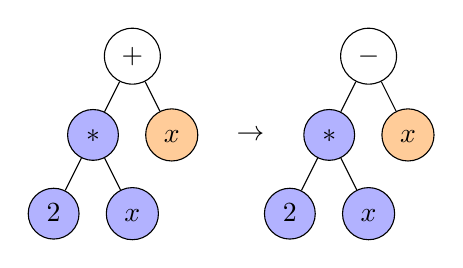
\begin{tikzpicture}
    \node[varnode] (del_plus) {$+$};
    \node[varnode, colorA] (del_times) at ($(del_plus)+(-0.5,-1)$) {$*$};
    \node[varnode, colorB] (del_one) at ($(del_plus)+(0.5,-1)$) {$x$};
    \node[varnode, colorA] (del_two) at ($(del_times)+(-0.5,-1)$) {$2$};
    \node[varnode, colorA] (del_three) at ($(del_times)+(0.5,-1)$) {$x$};
    \draw (del_plus) -- (del_times);
    \draw (del_plus) -- (del_one);
    \draw (del_times) -- (del_two);
    \draw (del_times) -- (del_three);

    \node[varnode] (ins_minus) at ($(del_plus)+(3,0)$) {$-$};
    \node[varnode, colorA] (ins_times) at ($(ins_minus)+(-0.5,-1)$) {$*$};
    \node[varnode, colorB] (ins_one) at ($(ins_minus)+(0.5,-1)$) {$x$};
    \node[varnode, colorA] (ins_two) at ($(ins_times)+(-0.5,-1)$) {$2$};
    \node[varnode, colorA] (ins_three) at ($(ins_times)+(0.5,-1)$) {$x$};
    \draw (ins_minus) -- (ins_times);
    \draw (ins_minus) -- (ins_one);
    \draw (ins_times) -- (ins_two);
    \draw (ins_times) -- (ins_three);

    \node (arrow) at ($(del_one)!0.5!(ins_times)$) {$\rightarrow$};
\end{tikzpicture}
\end{minipage}\hfill
\begin{minipage}{0.49\textwidth}
\centering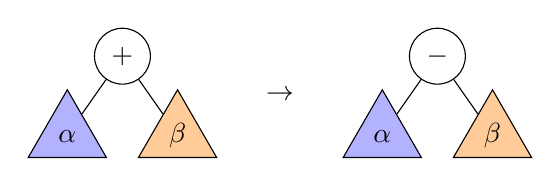
\begin{tikzpicture}
    \node[varnode] (del_plus) {$+$};
    \node[mvnode, colorA] (del_alpha) at ($(del_plus)+(-0.7,-1)$) {$\alpha$};
    \node[mvnode, colorB] (del_beta) at ($(del_plus)+(0.7,-1)$) {$\beta$};
    \draw (del_plus) -- (del_alpha);
    \draw (del_plus) -- (del_beta);

    \node[varnode] (ins_minus) at ($(del_plus)+(4,0)$) {$-$};
    \node[mvnode, colorA] (ins_alpha) at ($(ins_minus)+(-0.7,-1)$) {$\alpha$};
    \node[mvnode, colorB] (ins_beta) at ($(ins_minus)+(0.7,-1)$) {$\beta$};
    \draw (ins_minus) -- (ins_alpha);
    \draw (ins_minus) -- (ins_beta);

    \node (arrow) at ($($(del_beta)!0.5!(del_plus)$)!0.5!($(ins_alpha)!0.5!(ins_minus)$)$) {$\rightarrow$};
\end{tikzpicture}
\end{minipage}
\caption{The change $\change{(2*x)+x}{(2*x)-x}$ becomes $\change{\alpha+\beta} {\alpha-\beta}$ after meta-variable elision.}
\label{fig:metavar_elision}
\end{figure}

Figure~\ref{fig:metavar_elision} illustrate such an ellision for a change where the programmer just transformed a $+$ into a $-$. The subexpression $(2*x)$ is elided as $\alpha$ and the subexpression $x$ is elided as $\beta$, therefore the result only talks about the operator modification, and is a more generic change.

A given meta-variable can occur more that twice (at least once in deletion and once in insertion but maybe more). Therefore, code displacements have multiple sources and multiple targets, but a given meta-variable will always represent an identical code sub-tree. The fact that a given meta-variable can have multiple sources may seem unsatisfying, but it makes it possible to detect code displacements automatically without arbitrary choices. Moreover, thanks to that, we can easily revert a difference by simply exchanging the deleted and inserted trees.

As an example, the change $\change{x*y}{x+x}$ will be elided as $\change{\alpha*y}{\alpha+\alpha}$ because $x$ was duplicated.
Conversely, the reverse change $\change{x+x}{x*y}$ will become $\change{\alpha+\alpha}{\alpha*y}$ as it is hard to tell automatically from which $x$ the kept one comes from.

This code displacement notion is especially important for capturing refactoring in differences to merge them correctly with other commits later.

\paragraph{Grammar of syntactic differences} The notion of syntactic differences and common spine are generic with
respect to the actual syntax of the source language. For this reason,
our formal definition for the difference language is parameterized
with respect to the source language grammar.  Therefore, we write
$S(\overrightarrow{t}, \overrightarrow{s})$ for a constructor from the
source language syntax, with an arbitrary but fixed number of subtrees
($t$) and subsequences ($s$). For instance, one of the possible $S$
could be the language construction for conditional expression
\lstinline[mathescape]|if $t_{cond}$ { $\overrightarrow{s_{true}}$ } else { $\overrightarrow{s_{false}}$ }|
with one expression sub-tree and two nested sequences of instructions.

This gives the following grammar for difference trees:
\begin{align*}
tree &::= S(\overrightarrow{tree}, \overrightarrow{seqelt}) \typsep \id \typsep \change{change}{change}\\
seqelt &::= tree \typsep \mathst{change} \typsep \mathul{change}\\
change &::= S(\overrightarrow{change}, \overrightarrow{change}) \typsep \alpha\\
\end{align*}

We can see that difference trees are composed by spine elements ($S$ constructs), unchanged holes ($\square$) or local changes ($\change{d}{i}$). In their spine elements, if there are sequences, their elements can be either difference trees themselves, inserted new trees or deleted trees. To finish, inside inserted or deleted code, we can arbitrarily replace any subtree by a meta-variable.

\gb{Notations about deletion, insertion and $\square$ are now introduced in the overview}

\subsubsection{Applying syntactic differences}
\label{sec:diff_application}

We can see syntactic differences as partial functions turning a syntax
tree into another syntax tree.  The difference between $d$ and $i$ is
therefore a function that is at least mapping $d$ to $i$, but it is
also defined on some other trees sharing all the relevant structure
with $d$.

For a given difference and source program tree, we can use the following algorithm:

First align the difference spine and deleted nodes with the source program. Only matching syntax constructors align, if a non-matching one is found, the application fails (it means that the source tree is not inside the domain of the difference). For each meta-variable, we keep a corresponding subtree, initially undefined. When a source program subtree is aligned with a meta-variable, either the meta-variable was undefined, and we set it to the subtree, or it was already defined and we check that its current definition matches. This ensures that if a meta-variable occurs twice, it corresponds to the same subtree everywhere.

Then we return the difference spine and inserted nodes, replacing meta-variables with their previously computed subtrees.

\begin{figure}[ht]
\begin{minipage}{0.42\textwidth}
\centering\begin{tikzpicture}
    \node[varnode] (spine_block) {$\{\ldots\}$};
    \node[changenode, colorDel] (spine_stmt1) at ($(spine_block)+(-2.5,-1.6)$) {\tikz{
        \node[varnode] (del_stmt) {$\textbf{let}$};
        \node[varnode] (del_x) at ($(del_stmt)+(-0.5,-1)$) {$x$};
        \node[mvnode, blue] (del_three) at ($(del_stmt)+(0.5,-1)$) {\color{black}$\alpha$};
        \draw (del_stmt) -- (del_x);
        \draw (del_stmt) -- (del_three);
    }};
    \node[varnode] (spine_stmt2) at ($(spine_block)+(-0.25,-1.1)$) {$=$};
    \node[changenode, colorIns] (spine_stmt3) at ($(spine_block)+(2.5,-1.6)$) {\tikz{
        \node[varnode] (ins_stmt) at ($(ins_block)+(1,-1)$) {$=$};
        \node[varnode] (ins_z) at ($(ins_stmt)+(-0.5,-1)$) {$z$};
        \node[varnode] (ins_nine) at ($(ins_stmt)+(0.5,-1)$) {$9$};
        \draw (ins_stmt) -- (ins_z);
        \draw (ins_stmt) -- (ins_nine);
    }};{};
    \node[varnode] (spine_y) at ($(spine_stmt2)+(-0.75,-1)$) {$y$};
    \node[changenode] (change_y) at ($(spine_stmt2)+(0.75,-1)$) {\tikz{
        \node[varnode, colorDel] (x) {$x$};
        \node[mvnode, blue, colorIns] (five) at ($(x)+(1.2,0)$) {\color{black}$\alpha$};
        \node (arrow) at ($(x)!0.5!(five)$) {$\rightarrow$};
    }};
    \draw (spine_block) -- (spine_stmt1);
    \draw (spine_block) -- (spine_stmt2);
    \draw (spine_block) -- (spine_stmt3);
    \draw (spine_stmt2) -- (spine_y);
    \draw (spine_stmt2) -- (change_y);
\end{tikzpicture}
\end{minipage}
$\left(
\begin{minipage}{0.25\textwidth}
\centering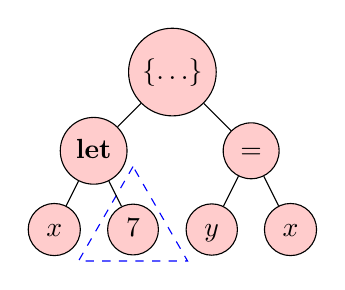
\begin{tikzpicture}
    \node[varnode, colorDel] (spine_block) {$\{\ldots\}$};
    \node[varnode, colorDel] (del_stmt) at ($(spine_block)+(-1,-1)$) {$\textbf{let}$};
    \node[varnode, colorDel] (del_x) at ($(del_stmt)+(-0.5,-1)$) {$x$};
    \node[varnode, colorDel] (del_three) at ($(del_stmt)+(0.5,-1)$) {$7$};
    \node[mvnode, dashed, minimum size=1.6cm, color=blue] (del_mv) at ($(del_stmt)+(0.5,-1)$) {};
    \draw (del_stmt) -- (del_x);
    \draw (del_stmt) -- (del_three);
    \node[varnode, colorDel] (spine_stmt2) at ($(spine_block)+(1,-1)$) {$=$};
    \node[varnode, colorDel] (spine_y) at ($(spine_stmt2)+(-0.5,-1)$) {$y$};
    \node[varnode, colorDel] (change_y) at ($(spine_stmt2)+(0.5,-1)$) {$x$};
    \draw (spine_block) -- (del_stmt);
    \draw (spine_block) -- (spine_stmt2);
    \draw (spine_stmt2) -- (spine_y);
    \draw (spine_stmt2) -- (change_y);
\end{tikzpicture}
\end{minipage}\right)$=
\begin{minipage}{0.25\textwidth}
\centering\begin{tikzpicture}
    \node[varnode, colorIns] (spine_block) {$\{\ldots\}$};
    \node[varnode, colorIns] (spine_stmt2) at ($(spine_block)+(-1,-1)$) {$=$};
    \node[varnode, colorIns] (ins_stmt) at ($(spine_block)+(1,-1)$) {$=$};
    \node[varnode, colorIns] (ins_z) at ($(ins_stmt)+(-0.5,-1)$) {$z$};
    \node[varnode, colorIns] (ins_nine) at ($(ins_stmt)+(0.5,-1)$) {$9$};
    \draw (ins_stmt) -- (ins_z);
    \draw (ins_stmt) -- (ins_nine);
    \node[varnode, colorIns] (spine_y) at ($(spine_stmt2)+(-0.5,-1)$) {$y$};
    \node[varnode, colorIns] (change_y) at ($(spine_stmt2)+(0.5,-1)$) {$7$};
    \node[mvnode, minimum size=1.6cm, color=blue] (del_mv) at ($(del_stmt)+(0.5,-1)$) {};
    \draw (spine_block) -- (spine_stmt2);
    \draw (spine_block) -- (ins_stmt);
    \draw (spine_stmt2) -- (spine_y);
    \draw (spine_stmt2) -- (change_y);
\end{tikzpicture}
\end{minipage}
\caption{The syntactic difference $\{\mathst{\mathbf{let}\ x=\alpha;}\ y = \change{x}{\alpha}; \mathul{z = 9}\}$ applied to $\{\mathbf{let}\ x=7;\ y = x\}$ gives $\{y = 7;\ z = 9\}$.}
\label{fig:apply_diff}
\end{figure}

On Figure~\ref{fig:apply_diff}, we can see that the tree applied to the difference correctly share relevant structure and the subtree $7$ matches the meta-variable $\alpha$. Therefore the result is shows a $7$ where the metavariable is inserted.

However, $3 + 4$ is not in the domain of neither $\change{3 - \alpha}{9 + \alpha}$ (non-matching constructions) nor $\change{\alpha + \alpha}{\alpha - \alpha}$ ($3$ and $4$ are different subtrees and cannot be both placed in the same meta-variable).

Appendix~\ref{app:diff_application_spec} shows a formal specification of the difference application.

\subsubsection{Computing a syntactic difference}
To compute a syntactic difference, we take syntax trees of both the original program and the modified program and we run the following algorithm:

\begin{enumerate}
  \item Compute a hash for each node of each syntax tree. This enables us to compare nodes in constant time later.

  \item Take the subset of hashes occurring both in original and
    modified syntax tree. Only the corresponding nodes occur in both trees, and are candidate for elision.

  \item Elide the nodes with a hash in the subset to remember just
    their hash.

  \item If an elided node does not match an elision with the same hash
    in the other tree, replace it by the original sub-tree. This ensures that every elided node occur at least once in both tree. The step is necessary because the subset of step 2 can contain nodes that are always below an ellided node, and therefore will not exist anymore.

  \item Merge both syntax trees into a common spine where possible (matching syntax constructors), else keep changes as two separate elided trees.
  Align sequences using recursively a dynamic algorithm minimizing the number of changed nodes of the resulting tree.
  Alignment is a refinement of the longest common subsequence problem  with variable cost for each unaligned element (number of changed nodes) and the possibility of aligning slightly different elements (recursively computing the alignments inside sub-trees and their costs).

  \item Replace each hash by a meta-variable letter (just an index in
    code), and replace changes $\change{\alpha}{\alpha}$ by $\id$ when $\alpha$ does not occur elsewhere. This step is only here to improve the presentation of the output.
\end{enumerate}

This algorithm is in $O(nm)$ where $n$ (resp. $m$) is the number of
node of the original (resp. modified) tree. The most computationally
expansive part of the algorithm is computing sequence alignments, all the rest is linear.

It is actually computing a difference between original and modified programs because we start from the trivial difference $\change{d}{i}$ and every step except step 3 does not lose any information. Step 3 elisions do not cause any trouble because step 4 only keep elisions that can be completed in presence of the source (or modified) program. By losing information, step 3 actually widens the domain of the final difference but does not change the result on tree $d$.

\subsection{Implementation considerations: extending syntax trees}
\label{sec:codegen}
Implementing an algorithm that requires extending a syntax tree can be tedious in practice because we want to attach new information and/or create holes on a fixed structure while keeping the typedness of the tree.

Along this paper, I give a Rust implementation for the syntax difference and merging algorithm of Rust programs. The parser used (the syn crate \cite{syn-crate}) uses more than 180 types in its syntax trees, so manual extension was not an option.

The solution I give is based on a somehow generic code generation system (implemented as procedural macro). The idea is that we want to add the ability to extend a type family of mutually recursive sum of products (nested enums and structs in Rust terminology) by systematically changing some types by others, thus generating a new family variant. Then, we also make a code generator to traverse or convert between variants of the same family. After generation, we only have to write manual code once for each new capability of the family variants.

See Appendix~\ref{app:codegen} for an example of how to use such code generator in practice. The code of the full project (including the code generator and the merging algorithm) can be found at \url{https://gaufre.informatique.univ-paris-diderot.fr/Bertholon/mergeory}.

Note that for having a production ready tool, the current parser is
not adapted, as it systematically forgets the comments inside source
code. But this is left for future work as a pure engineering problem.

\subsection{Awareness colors}
\label{sec:colors}
Before merging differences together, we want to define a way of keeping track of which commit introduced each modification. For that we use a notion of awareness colors.

Each commit in a fusion gets an associated tint. If we denote by
$\mathbb{T}$ the set of all tints considered, we can define the color
set as $\mathbb{C} = \mathcal{P}(\mathbb{T})$. This forms the complete
lattice $(\mathbb{C}, \cup, \cap, \subset)$. We name the maximum in
this lattice white (equal to $\mathbb{T}$, denoted by $\top$) and the
minimum black (equal to $\emptyset$, denoted by $\bot$).

A change gets the color $c \in \mathbb{C}$, if for all
tint in $c$, the associated commit is aware of the behavior (new and broken invariants) of the colored source code. \yrg{You already
used $c$ in the syntax for differences!}\gb{Not anymore}
Similarly, a value has a color $c \in \mathbb{C}$ if for all tints in $c$, the corresponding commit is fully aware of it, or at least aware of all the meaningful invariants inside it.

The white color having all the tints, it represent a consensus of all the commits. On the other side, black represent the fact that no single commit can claim responsibility alone for a given value or code. This makes the white color the good choice for everything already present in the original program, and black a color that we want to track and avoid because it represent an ambiguity.

All changes carry a color. We denote by $\mathul{code}^c$ (resp. $\mathst{code}^c$) an insertion (resp. deletion) carrying color $c$. In examples and figures we use actual colors ($\setstcolor{orange}\mathst{code}$ or $\color{orange}\mathul{code}$) instead\footnote{For obvious practical reasons, terms with white color are written in black (I would like a dark paper background but it doesn't print well...). Fortunately, black is never directly written in this notation.}.

If the exact same modification is done twice, the result has the union of tints as its color as any of the two commits know the modification.

\newbox\boxdelinner
\sbox\boxdelinner{\setul{-.75ex}{}$\mathul{x}^c$}
\newbox\boxinsinner
\sbox\boxinsinner{\setul{.1ex}{}$\mathul{x}^c$}
However, insertions and deletion do not behave exactly in the same way regarding composition. If some code is deleted inside deleted code, the color of the deletion is the union of the colors ($\setul{-.4ex}{}\mathul{\usebox\boxdelinner}^{c'} = \mathst{x}^{c \cup c'}$) because any of the two modifications can be held responsible for the deletion. However, if some code is inserted inside inserted code, we have to consider the intersection of the colors ($\setul{.4ex}{}\mathul{\usebox\boxinsinner}^{c'} = \mathul{x}^{c \cap c'}$) because only the interaction between the modifications explain the final behavior. These composition cases occur mainly in presence of meta-variables or during execution (see section \ref{sec:colored-diff-oracle}).

Before merging, we apply the singleton color corresponding to the
commit on the difference tree, recursively as follows:
\begin{align*}
{\color{orange}tree} &= S(\overrightarrow{\color{orange}tree}, \overrightarrow{\color{orange}seqelt}) \typsep \id \typsep {\setstcolor{orange}\setulcolor{orange}\change{change}{\color{orange}change}}\\
{\color{orange}seqelt} &= {\color{orange}tree} \typsep {\setstcolor{orange}\mathst{change}} \typsep {\color{orange}\mathul{change}}\\
{\color{orange}change} &= {\color{orange}S(\overrightarrow{change}, \overrightarrow{change})} \typsep {\color{orange}\alpha}\\
\end{align*}

Note that unchanged parts are never colored, and that syntax nodes are not colored in the spine but are in the changed sub-trees. This reflects the fact that in the spine and inside holes, code comes from the original source code, while elsewhere it is introduced by the commit. \yrg{I am wondering if you should not use the background color to colorize terms...}\gb{Combining background would be hard, while in the overview example I double strike-trough and give distinct colors inside changes}

\subsection{Merging differences}
Now that we have difference trees for each individual concurrent
change, we can try to merge them in a way that keeps track of the
origin of each piece of code.

\subsubsection{High-level specification of a merging algorithm}
A merging algorithm takes two differences and produce another difference that contains all the changes from inputs if they are compatible or show where they are incompatible otherwise. This high-level description is underspecified because semantically combining changes only has an intuitive meaning depending on the implicit idea of what each commit does (often summarized in English in the commit message). Therefore, these algorithms are necessarily somehow arbitrary because they force a particular meaning for change combination. This does not mean that they are all equivalent, their definition for combination is more or less aligned with usual real-life commits.

In this paper, our arbitrary choice is to focus on syntax to align differences (because we think that it often follows the intuition of the developers) and let changes follow moved code (because it allow seamless merging of a large class of refactoring operations). These two principles will be explained further in Section~\ref{sec:merge_principles}. That said, we avoid further arbitrary choices that could favor one of the input tree over the other.

\yrg{At this point, you must discuss what are
  the design principles that guided your work to get a form of
  syntactical merge which seems to take no arbitrary choice at the
  level of syntax...}\gb{Hmm, you mean low level principles like merge common spine or push meta-variables down the deletion trees? This seems too 'low-level' for this part...}

We will denote $t_1 \merge t_2$ the result of our merge algorithm on difference trees $t_1$ and $t_2$.
  
Often the two input differences will not share the same domain. The output can therefore only be defined on the intersection of these domains. It makes no sense to merge differences whose domain are disjoint. In a standard setup, both input differences were computed on a common base and therefore we are sure that the merge output is at least defined for this base program.

On top of that, the merging operation can and will regularly produce conflicts whenever someone wants to merge syntactically incompatible changes.
Therefore we need to extend our grammar of differences to include these conflicts. Insertions and deletions do not trigger the same kind of conflicts, so we have to break the symmetry between them. It leads to the following grammar:
\begin{align*}
tree &::= S(\overrightarrow{tree}, \overrightarrow{seqelt}) \typsep \id \typsep  \change{del}{ins}\\
seqelt &::= tree \typsep \mathst{del} \typsep \DelConflict(del, ins) \typsep \mathul{ins} \typsep \OrdConflict(\overrightarrow{\overrightarrow{ins}})\\
del &::= S(\overrightarrow{del}, \overrightarrow{del}) \typsep \alpha \typsep \MvConflict(\alpha, del, ins) \\
ins &::= S(\overrightarrow{ins}, \overrightarrow{insseqelt}) \typsep \alpha \typsep \InsConflict(\overrightarrow{ins})\\
insseqelt &::= ins \typsep \DelConflict(ins) \typsep \OrdConflict(\overrightarrow{ins})\\
\end{align*}

Conflict represent parts that couldn't be merged and therefore prevent application of the difference on any tree. They can come from four different sources:
\begin{itemize}
  \item Insertion conflict ($\InsConflict$) simply represent two different insertions that were about to be merged in the same place.
  \item Deletion conflict ($\DelConflict$) appears where one commit deletes a node while the other one had changes in it.
  \item Insert order conflict ($\OrdConflict$) is caused by two insertions taking place at the same location. As the merge operation is never performing any choice, it cannot arbitrarily order them.
  \item Meta-variable conflict ($\MvConflict$) is triggered when a meta-variable appears more than once in deletion tree, and the inlined insertions in each occurrences differ, therefore not giving a consistent replacement. This will be explained in further details later.
\end{itemize}

As this syntax is an extension, the syntax differences presented earlier can be directly reinterpreted in this grammar and conversely, differences without conflicts still follow the old grammar. Moreover, these new trees are also colored. \gb{Should I color the grammar?}

\subsubsection{Design principles for our merging algorithm}
\label{sec:merge_principles}
\paragraph{Align changes following the syntax}
As the domains of both input differences must overlap, we always can align their spine and deletion trees. This therefore also give a full change alignment as insertions are attached on a specific place in the spine (however it sometimes creates conflicts). By doing so, we respect the property that no commit is favored because alignment comes from shared nodes.

The first step of the merging algorithm aligns the common spine nodes and unwind the remaining ones that are facing a change. On Figure~\ref{fig:spine_alignment}, we can see that only the nodes $x$ and $+$ are in both spines. Therefore, spine nodes $y$ and $*$ in the orange tree must be unwinded producing white nodes as a change before merging.

\begin{figure}[ht]
\begin{minipage}{0.33\textwidth}
\centering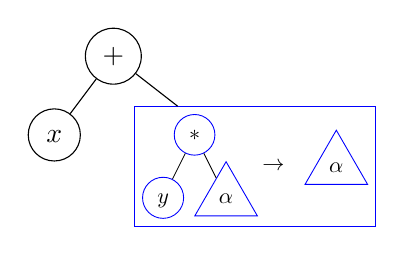
\begin{tikzpicture}
\node[varnode] (plus) {$+$};
\node[varnode] (x) at ($(plus)+(-0.75,-1)$) {$x$};
\node[changenode, color=blue] (change) at ($(plus)+(1.8,-1.4)$) {\tikz[color=black]{
    \node[varnode, color=blue] (del_times) {$\color{black}*$};
    \node[varnode, color=blue] (del_y) at ($(del_times)+(-0.5,-1)$) {$\color{black}y$};
    \node[mvnode, color=blue] (del_alpha) at ($(del_times)+(0.5,-1)$) {$\color{black}\alpha$};
    \draw (del_times) -- (del_y);
    \draw (del_times) -- (del_alpha);
    
    \node[mvnode, color=blue] (ins_alpha) at ($(del_times)!0.5!(del_alpha)+(2, 0)$) {$\color{black}\alpha$};
    \node (arrow) at ($(del_times)!0.5!(del_alpha)!0.5!(ins_alpha)$) {$\rightarrow$};
}};
\draw (plus) -- (x);
\draw (plus) -- (change);
\end{tikzpicture}
\end{minipage}\hfill
\begin{minipage}{0.33\textwidth}
\centering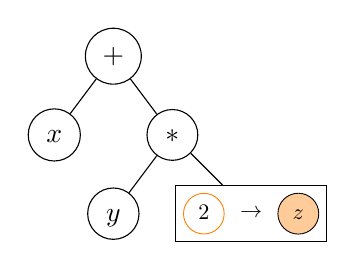
\begin{tikzpicture}
\node[varnode] (plus) {$+$};
\node[varnode] (x) at ($(plus)+(-0.75,-1)$) {$x$};
\node[varnode] (times) at ($(plus)+(0.75,-1)$) {$*$};
\node[varnode] (y) at ($(times)+(-0.75,-1)$) {$y$};
\node[changenode] (change) at ($(times)+(1,-1)$) {\tikz{
    \node[varnode, color=orange] (two) {$\color{black}2$};
    \node[varnode, colorB] (z) at ($(two)+(1.5, 0)$) {$z$};
    \node (arrow) at ($(two)!0.5!(z)$) {$\rightarrow$};
}};
\draw (plus) -- (x);
\draw (plus) -- (times);
\draw (times) -- (y);
\draw (times) -- (change);
\end{tikzpicture}
\end{minipage}
\hfill
\begin{minipage}{0.33\textwidth}
\centering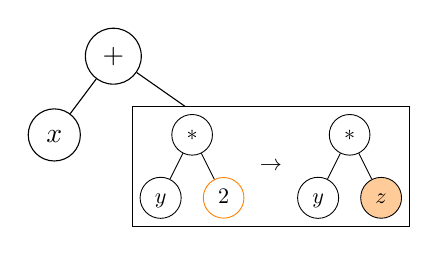
\begin{tikzpicture}
\node[varnode] (plus) {$+$};
\node[varnode] (x) at ($(plus)+(-0.75,-1)$) {$x$};
\node[changenode] (change) at ($(plus)+(2,-1.4)$) {\tikz{
    \node[varnode] (del_times) {$\color{black}*$};
    \node[varnode] (del_y) at ($(del_times)+(-0.5,-1)$) {$\color{black}y$};
    \node[varnode, color=orange] (del_two) at ($(del_times)+(0.5,-1)$) {$\color{black}2$};
    \draw (del_times) -- (del_y);
    \draw (del_times) -- (del_two);
    
    \node[varnode] (ins_times) at ($(del_times)+(2.5, 0)$) {$*$};
    \node[varnode] (ins_y) at ($(ins_times)+(-0.5,-1)$) {$y$};
    \node[varnode, colorB] (ins_z) at ($(ins_times)+(0.5,-1)$) {$z$};
    \draw (ins_times) -- (ins_y);
    \draw (ins_times) -- (ins_z);
    
    \node (arrow) at ($($(del_times)!0.5!(del_two)$)!0.5!($(ins_times)!0.5!(ins_y)$)$) {$\rightarrow$};
}};
\draw (plus) -- (x);
\draw (plus) -- (change);
\end{tikzpicture}
\end{minipage}
\caption{Spine alignment: We unwind the spine of the second tree producing the third in order to be aligned with first.}
\label{fig:spine_alignment}
\end{figure}

If a difference sub-tree is aligned with an unchanged node (either $\square$ or $\change{\alpha}{\alpha}$), we keep the changed one only. This is quite an intuitive notion of combination with unchanged node yielding to the important property $t \merge \square = t$.

When merging deletion trees, either both inputs agree on a common syntax node, or one of them has a meta-variable. In the latter case, we have to produce the most specific deletion tree, therefore keeping the non meta-variable sub-tree. This is the consensus between the two differences as the one with meta-variable accepts any sub-tree at this point while the other accepts only the kept one. We must remember that the meta-variable has been deleted for a more specific tree and replace its remaining occurences in deletions (always) and insertions (except in case of the inlining explained later).

\gb{I probably should add an example here, but it is hard to find one that is non-conflicting, not complex and without inlining}

When merging insertion trees, however, meta-variables always conflict with each other because they correspond to specific subtrees instead of capturing one. Therefore, we only merge fully identical nodes.

\paragraph{Inlining changes inside meta-variables}
When dealing with meta-variables, that represent a multi-source
multi-target code move, our merging algorithm will try to push changes
toward the destination of the code movement.

This is done in a two-phase way. First, if we have two changes facing each other we try to inline one of them inside the deletion tree of the other, by allowing differences wherever we have a meta-variable. By doing so, we check if the changes of one difference are fully contained inside code that will be moved by the other.

Then, we check that these inlined changes are consistent across different occurrences of the same meta-variable. If they are, we replace all occurrences of the meta-variable by the obtained insertion. If they are not, we generate a $\MvConflict$ conflict on each deleted $\alpha$ with the corresponding facing insertion.

\begin{figure}[ht]
\begin{minipage}{0.49\textwidth}
\centering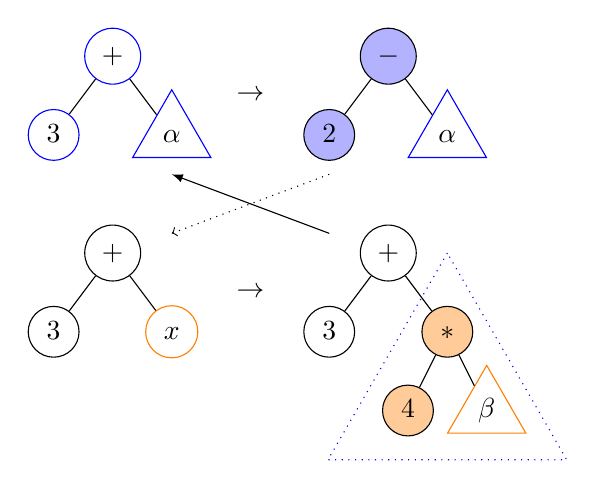
\begin{tikzpicture}
    \node[varnode, color=blue] (adel_plus) {$\color{black}+$};
    \node[varnode, color=blue] (adel_three) at ($(adel_plus)+(-0.75,-1)$) {$\color{black}3$};
    \node[mvnode, color=blue] (adel_alpha) at ($(adel_plus)+(0.75,-1)$) {$\color{black}\alpha$};
    \draw (adel_plus) -- (adel_three);
    \draw (adel_plus) -- (adel_alpha);

    \node[varnode, colorA] (ains_minus) at ($(adel_plus)+(3.5,0)$) {$-$};
    \node[varnode, colorA] (ains_two) at ($(ains_minus)+(-0.75,-1)$) {$2$};
    \node[mvnode, color=blue] (ains_alpha) at ($(ains_minus)+(0.75,-1)$) {$\color{black}\alpha$};
    \draw (ains_minus) -- (ains_two);
    \draw (ains_minus) -- (ains_alpha);

    \node (aarrow) at ($($(adel_alpha)!0.5!(adel_plus)$)!0.5!($(ains_two)!0.5!(ains_minus)$)$) {$\rightarrow$};
    
    \node[varnode] (bdel_plus) at ($(adel_plus)+(0,-2.5)$) {$+$};
    \node[varnode] (bdel_three) at ($(bdel_plus)+(-0.75,-1)$) {$3$};
    \node[varnode, color=orange] (bdel_x) at ($(bdel_plus)+(0.75,-1)$) {$\color{black}x$};
    \draw (bdel_plus) -- (bdel_three);
    \draw (bdel_plus) -- (bdel_x);

    \node[varnode] (bins_plus) at ($(bdel_plus)+(3.5,0)$) {$+$};
    \node[varnode] (bins_three) at ($(bins_plus)+(-0.75,-1)$) {$3$};
    \node[varnode, colorB] (bins_times) at ($(bins_plus)+(0.75,-1)$) {$*$};
    \node[varnode, colorB] (bins_four) at ($(bins_times)+(-0.5,-1)$) {$4$};
    \node[mvnode, color=orange] (bins_beta) at ($(bins_times)+(0.5,-1)$) {$\color{black}\beta$};
    \node[mvnode, dotted, minimum size=3.5cm, color=blue] (bins_alpha) at ($(bins_times)+(0,-0.75)$) {};
    \draw (bins_plus) -- (bins_three);
    \draw (bins_plus) -- (bins_times);
    \draw (bins_times) -- (bins_four);
    \draw (bins_times) -- (bins_beta);
    
    \node (barrow) at ($($(bdel_x)!0.5!(bdel_plus)$)!0.5!($(bins_three)!0.5!(bins_plus)$)$) {$\rightarrow$};
    
    \draw[>=latex,->] ($(bins_plus)+(-0.75, 0.25)$) -- ($(adel_alpha)+(0, -0.5)$);
    \draw[->,dotted] ($(ains_two)+(0, -0.5)$) -- ($(bdel_plus)+(0.75, 0.25)$);
\end{tikzpicture}
\end{minipage}\hfill
\begin{minipage}{0.49\textwidth}
\centering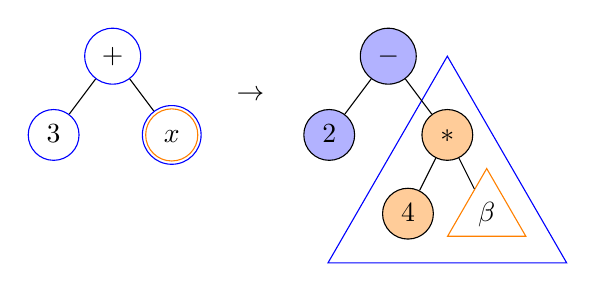
\begin{tikzpicture}
    \node[varnode, color=blue] (del_plus) {$\color{black}+$};
    \node[varnode, color=blue] (del_three) at ($(del_plus)+(-0.75,-1)$) {$\color{black}3$};
    \node[varnode, color=orange] (del_x) at ($(del_plus)+(0.75,-1)$) {$\color{black}x$};
    \node[varnode, color=blue] (del_x_out) at (del_x) {\phantom{M}};
    \draw (del_plus) -- (del_three);
    \draw (del_plus) -- (del_x_out);

    \node[varnode, colorA] (ins_minus) at ($(del_plus)+(3.5,0)$) {$-$};
    \node[varnode, colorA] (ins_two) at ($(ins_minus)+(-0.75,-1)$) {$2$};
    \node[varnode, colorB] (ins_times) at ($(ins_minus)+(0.75,-1)$) {$*$};
    \node[varnode, colorB] (ins_four) at ($(ins_times)+(-0.5,-1)$) {$4$};
    \node[mvnode, color=orange] (ins_beta) at ($(ins_times)+(0.5,-1)$) {$\color{black}\beta$};
    \node[mvnode, minimum size=3.5cm, color=blue] (ins_alpha) at ($(ins_times)+(0,-0.75)$) {};
    \draw (ins_minus) -- (ins_two);
    \draw (ins_minus) -- (ins_times);
    \draw (ins_times) -- (ins_four);
    \draw (ins_times) -- (ins_beta);

    \node (arrow) at ($($(del_x)!0.5!(del_plus)$)!0.5!($(ins_two)!0.5!(ins_minus)$)$) {$\rightarrow$};
\end{tikzpicture}
\end{minipage}
\caption{Example of successful meta-variable inlining}
\label{fig:metavar_inlining}
\end{figure}

On Figure~\ref{fig:metavar_inlining}, we can see that the orange change can be inlined in the blue deletion tree. Indeed, if we compare their tree, all differences occur under meta-variable $\alpha$. Conversely, the blue change cannot be inlined because the inserted node $-$ in blue cannot be merged with deleted node $+$ in the orange tree. If there are no other occurrences of $\alpha$, or the corresponding inlined tree is always $4*\beta$, we can replace every $\alpha$ by $4*\beta$, producing the tree on the right.

To avoid making any arbitrary choice, meta-variable inlining is ignored if both changes could be inlined in the other. This brings back the important property that merging a change with itself does not change anything.

\paragraph{Color propagation}
While merging, we propagate the colors that are on the input nodes to the output. To do so we follow the discipline described in Section~\ref{sec:colors}, without any difficulties. When code replace a meta-variable because of inlining, it keeps its original color but is now under an insertion context that also have the color of the original meta-variable. By color composition rule, this is the only way to create black color during the syntactic phase. One could notice that meta-variable inlining will often create black colors that we want to avoid. This is intended as color ambiguities are a lot easier to resolve than syntactic conflicts.

\subsubsection{Algorithm for merging differences}
\label{sec:syntactic_merge_algo}

\gb{Cette section reste très technique, mais je ne pense pas pouvoir y échapper...}
Following the principles exposed above, our algorithm follows these steps:
\begin{enumerate}
 \item Ensure that all the meta-variables used in both programs are
   disjoint by alpha-renaming whenever necessary. This prevent merging different similarly named meta-variables that correspond to different subtrees.

 \item Align the spines of both difference trees as explained in Section~\ref{sec:merge_principles}. This step also aligns the sequences in the spine and detects insert order conflicts.
 
 \item Merge the facing insertion trees together. This can only occur when two in-tree modifications face each other: $(\change{d_l}{i_l}) \merge (\change{d_r}{i_r})$ (otherwise, insertions are processed at step 2 because they are either identical or conflict for ordering).
 In that case try to perform inlinings of $i_l$ into $d_r$ and $i_r$ into $d_l$. If exactly one succeeds, let's say $i_l$, remember inside $d_r$ the associations $i_l$ subtree / $d_r$ meta-variable as temporarily $\MvConflict$ conflict and keep $i_r$ alone as the merged insertion. Else, recursively align $i_l$ with $i_r$, yielding $\OrdConflict(i_l, i_r)$ on (sub)nodes that were distinct.
 
 To ease checking later, during this step, we keep for each meta-variable $\alpha$ a list $\Gamma^*(\alpha)$ of sub-trees that were inlined inside it, and remember which meta-variables occurred in a failed inlining.

 \item Merge the facing deletion trees together. For that we align deleted trees with each other. If they do not match, we can stop here as it means that the domain intersection of inputs is empty. 
 
 When we align a subtree with a meta-variable, we need later to remove the meta-variable everywhere. For that we remember $\Delta$ a map from meta-variables to deletion sub-tree replacements. If there is a subsequent alignment with a meta-variable $\alpha$ whose replacement in $\Delta$ is already filled, we continue alignment with $\Delta(\alpha)$. If we encounter $\MvConflict$ nodes, we simply traverse them.

 \item Perform the substitutions wherever there are meta-variables with a replacement in $\Delta$ for deletion trees, and in $\Gamma$ for insertion trees. Note that some meta-variables are not removed in the merge process and therefore do not occur in $\Delta$ or $\Gamma$. We do so by browsing once again all the partially merged difference.
 
 $\Gamma$ is a meta-variable replacement function computed on the fly from $\Gamma^*$. For a meta-variable $\alpha$ that never occurs in failed inlining, if all elements of $\Gamma^*(\alpha)$ are equal to the same insertion tree $i$, then $\Gamma(\alpha) = i$ else we have $\Gamma(\alpha) = \top$. Having all elements of $\Gamma^*(\alpha)$ equal means that the replacement is coherent across the various occurrences of $\alpha$. For a meta-variable that occurs in failed inlining then $\Gamma(\alpha)$ is an white insertion tree version of $\Delta(\alpha)$ when $\Gamma^*(\alpha)$ is empty and $\top$ otherwise. This makes sense because when a meta-variable is never inlined into, we should expand it in insertions as 
 When $\Gamma(\alpha) = \top$, we never replace $\alpha$ and we keep the related $\MvConflict$ structures in deletion trees. Else, we remove these $\MvConflict$ structures as the ``conflict'' does not exist because inlining has been fully resolved.
 
 Substitutions inside substitutions may be required. So we first substitute inside $\Delta$ and $\Gamma$ before replacing a meta-variable. This can lead to cycles on edge cases. We resolve cycles in $\Gamma$ as $\top$ because we want to keep conflicts on degenerate cases, and in $\Delta$ as a fresh meta-variable because we can notice that cycles only occur for meta-variables aliasing each other (otherwise only infinitely long syntax tree would be in the domain intersection).
\end{enumerate}

This algorithm is implemented (in the repository mentioned Section~\ref{sec:codegen}) but not fully formalized yet. You can find an unfinished formal specification in Appendix~\ref{app:syntactic_merge_spec}.

\subsubsection{Properties of the generated merged difference tree}
\label{sec:merge_properties}
Despite the rather arbitrary choice of doing this specific syntactic
merge, our algorithm should eventually provide some good
properties. These properties are not proved, but follow from the design principles.

\paragraph{Preserve common spine}
All the nodes that are inside the spine of both commits are preserved.

\paragraph{Deletion tree intersection}
If some code is deleted in one of the commits with color $c$, it must also be deleted in the merged result with a color $c' \supseteq c$.

\paragraph{Domain}
We can notice that in absence of conflicts, the domain of the
merged difference is the intersection of the domains of both
inputs. Mathematically, we have: $\dom(t_1 \merge t_2) = \dom(t_1)
\cap \dom(t_2)$. This comes from spine preservation combined with
deletion tree intersection.
\yrg{Notice that you never formally defined the domain of the
merged difference.}\gb{Isn't the interpretation of differences as functions from \ref{sec:diff_application} implicitly defining it?}

\paragraph{Idempotence}
$t \merge t = t$. This comes from the fact that we do not let
conflicts or change inlining happen when both inputs agree on a common value. The property can be extended to differently colored tree as: $t^{c_1} \merge
t^{c_2} = t^{c_1 \cup c_2}$.

\paragraph{Commutativity}
$t_1 \merge t_2 = t_2 \merge t_1$, this shows that we cannot treat differently the left and the right commits, thus never favoring one side against the other. There is a little limitation though, we must consider that the order inside
conflicts does not matter: $\InsConflict(i_1, i_2) = \InsConflict(i_2,
i_1)$, $\OrdConflict([\overrightarrow{i}]) =
\OrdConflict(\sigma[\overrightarrow{i}])$ for any permutation $\sigma$
and $\MvConflict(\alpha, \MvConflict(\beta, d, i_\beta), i_\alpha) =
\MvConflict(\beta, \MvConflict(\alpha, d, i_\alpha), i_\beta)$.

\paragraph{Preserve introduced nodes}
For all nodes that are introduced in one of the commits, we know that it will be found at least once in the merged result. However, we cannot say anything about location of these introduced nodes because their code might have been displaced by meta-variable inlining.

\paragraph{Compatible with composition}
We denote by $\circ$ the sequential composition of changes: this means that $(t_1 \circ t_2)(d) = t_1(t_2(d))$. Note that the domain of such composition might be empty.
If $d \in \dom(t_1 \circ t_2)$ and $t_1 \circ t_2 = t_2 \circ
t_1$, we have $(t_1 \merge t_2)(d) = (t_1 \circ t_2)(d)$. Here the
precondition will be true for differences without code moves. This
means that on orthogonal changes, the merge operation is the same as
the composition where they are both defined. \todo{Check that we
  cannot remove the domain assumption}\gb{This check is out of scope with the time I have left...}

\paragraph{Compatible with inverse}
If $d \in \dom(t_1^{-1} \circ (t_1 \merge t_2))$, then $(t_1^{-1}
\circ (t_1 \merge t_2))(d) = t_2(d)$. Note here that inverse is
defined for differences without colors, so the equality holds only
after removing all colors from $t_1$ and $t_2$. This is less powerful as one may think, because often, $\dom(t_1^{-1} \circ (t_1 \merge t_2))$ will be empty.

\subsection{Self-contained difference}

If we want to merge more than two differences, we can reapply the same
algorithm on already merged trees, thus accumulating modifications but
also conflicts.

In a setup where all commits come from a common base, when all relevant commits are accumulated and before moving on to the semantic analysis, we replace all the meta-variables and holes that are left in the merged difference with their associated code in the common base to produce a self-contained file. This pseudo-applied difference, allows us to retrieve both the base code and the merged code but also keeps the colors and the position of the changes. Therefore it is a good input format for the semantic analysis.

\todo{Grammar of this format if space is available. I doubt about this...}

\section{Checking and restoring the semantic of merged program}
\label{sec:semantic-merge}

Having two commits syntactically merged does not mean that the result
is a valid semantic combination that respect the intentions of all
original committers. We can see an example of such collision in Listing~\ref{lst:double-incr}.

\begin{lstlisting}[label=lst:double-incr, caption={Double fix of the same function by different commits. The syntactic fusion does not create a conflict but semantically we will most probably create a bug here.}]
fn compute_something(x: i32) -> i32 {
    let mut a = x * x;
    @\color{blue}\ul{a += 1;}@
    @\setstcolor{orange}\st{a} $\rightarrow$ {\color{orange}\ul{a + 1}}@
}
\end{lstlisting}

That is why after the syntax merging step, we also want to check the
semantic of the fusion for possible ambiguities.

In this section, we first will show that self-contained
non-conflicting difference trees can be interpreted as correlation
oracles~\cite{girka2017verifiable} between the original code and a merged candidate,
that is specific relation between the two programs' execution
traces. Secondly, we show that we can derive a runtime analysis that
ensures that there is no unresolved ambiguity introduced by the fusion
operation. In future work, this runtime analysis could be refined into
a static analysis. Finally, we will describe a possible conflict resolution system that interacts with our analysis.

\subsection{Operational semantics of the studied language}

In this paper, we will use a simplified version of the Rust
programming language~\cite{rust-lang}. We chose this language because it
allows us to explore both functional and imperative coding styles.  We ignore all the borrowing and trait systems that could be difficult to understand for a reader without any Rust background.

\newcommand{\ident}{\mathbb{I}}
\newcommand{\typ}{\mathbb{T}}

Syntactically, with $\ident$ the set of variable and function
identifiers, $\typ$ the set of type identifiers, $\diamond$
(resp. $\star$) the set of primitive binary (resp. unary) functions, and $\boxed{a}^*$ the repetition of zero or more times $a$,
the syntax for our toy language is defined by the following grammar:
\begin{align*}
program &::= \boxed{item}^*\\
item &::= func \typsep enum\\
enum &::= \mathbf{enum}\ \typ\ \{ \boxed{\ident(\boxed{\typ,}^*),}^* \}\\
func &::= \mathbf{fn}\ \ident(\boxed{\ident: \typ}^*) \rightarrow \typ\ block\\
block &::= \{ \boxed{expr;}^* expr \}\\
expr &::= \ident \typsep literal \typsep \star expr \typsep expr \diamond expr \typsep \ident = expr \typsep \ident(\boxed{expr,}^*) \typsep block\\
&\typsep \mathbf{if}\ expr\ block\ \mathbf{else}\ block \typsep \mathbf{while}\ expr\ block \typsep \mathbf{match}\ expr\ \{ \boxed{\ident(\boxed{\ident,}^*) \Rightarrow expr,}^* \}\\
&\typsep \mathbf{continue} \typsep \mathbf{break} \typsep \textbf{return}\ expr\\
literal &::= () \typsep \mathbf{true} \typsep \mathbf {false} \typsep \mathbb{Z}\\
value &::= literal \typsep \ident(\boxed{value,}^*)\\
\end{align*}

\yrg{What do the boxes mean? Is that a standard format? If so, could
  you give a reference for its specification?} \gb{It comes from the documentation of Coq apparently. I added its introduction above the definition.}

\yrg{What is the meaning of $\star expr$?} \gb{It is written above... Don't know how to improve.}

To define the semantics, we define the program state as a tuple
$\rtstate{\kappa}{v}{S}$ where $\kappa$ is the continuation, $v$ the
value of the last computed expression and $S$ the local store
stack.
The value of the last computed expression is needed in program states because any expression can itself be a complex branching subprogram returning the value we need to continue (as functionnal programming style requires). Instructions in continuation refer to this previous value with the pseudo-expression $\square$.
When a function is called, we push a new store on top of the previous
one. Only the topmost store can be used and updated as it
corresponds to the stack frame of the current function.
For simplicity reasons, our language does not feature references, so the heap is omitted, however it should work similarly to a global store indexed by adresses.

We also keep the set of constructors, and the set of functions as a
global state.\footnote{Technically, we could say that named functions are constants of the global environment and that there exist a meta-language operation extracting the code out of a function value into colored continuation elements. As this induce more complexity in the explanations we stick to first-order programs (no anonymous lambda abstraction).}
\yrg{That global environment is hardly compatible with a
  higher-order language, right? That's fine because your language is
  first order. Yet, the introduction
  emphasizes that you chose a sublanguage of Rust to play with
  functional programs: this looks a bit contradictory.}\gb{See footnote. This paper is way too technical already. When I said that we chose Rust for functional behaviors, I was mostly thinking of algebraic datatypes and of the ``every piece of code yields a value'' idiom} We denote
$\mathbb{G}(f)$ the body of function $f$ taken from global
state. Types do not play any role in reduction rules, but we will
assume that programs are already well typed. The initial state is
given by the call of the entry point function $f$ with its arguments
$\overrightarrow{x_a}$:
$\rtstate{\mathbb{G}(f)}{()}{\{\overrightarrow{x_a \leftarrow
    v_a}\}}$.

Then, if we denote by $\kappa_{\neg \mathbf{kw}}$ any sequence of instructions without the keyword $\mathbf{kw}$, the program follows the reduction rules below:
\begin{align*}
\rtstate{\{\overrightarrow{e_s;}\ e\} \cdot \kappa}{v}{S} &\rightarrow \rtstate{\overrightarrow{e_s} \cdot e \cdot \kappa}{()}{S}\\
\rtstate{x = e \cdot \kappa}{v}{S} &\rightarrow \rtstate{e \cdot x = \square \cdot \kappa}{()}{S}\\
\rtstate{x = \square \cdot \kappa}{v}{S} &\rightarrow \rtstate{\kappa}{()}{S[x \leftarrow v]}\\
\rtstate{x \cdot \kappa}{v}{S} &\rightarrow \rtstate{\kappa}{S(x)}{S}\\
\rtstate{literal \cdot \kappa}{v}{S} &\rightarrow \rtstate{\kappa}{literal}{S}\\
\rtstate{\star e \cdot \kappa}{v}{S} &\rightarrow \rtstate{e \cdot \star \square \cdot \kappa}{()}{S}\\
\rtstate{\star \square \cdot \kappa}{v}{S} &\rightarrow \rtstate{\kappa}{\star v}{S}\\
\rtstate{e_1 \diamond e_2 \cdot \kappa}{v}{S} &\rightarrow \rtstate{e_1 \cdot \square \diamond e_2 \cdot \kappa}{()}{S}\\
\rtstate{\square \diamond e_2 \cdot \kappa}{v}{S} &\rightarrow \rtstate{e_2 \cdot v \diamond \square \cdot \kappa}{()}{S}\\
\rtstate{v_1 \diamond \square \cdot \kappa}{v_2}{S} &\rightarrow \rtstate{\kappa}{v_1 \diamond v_2}{S}\\
\rtstate{\varphi(\overrightarrow{v_a}, e, \overrightarrow{e_r}) \cdot \kappa}{v}{S} &\rightarrow \rtstate{e \cdot \varphi(\overrightarrow{v_a}, \square, \overrightarrow{e_r}) \cdot \kappa}{()}{S}\\
\rtstate{\varphi(\overrightarrow{v_a}, \square, \overrightarrow{e_r}) \cdot \kappa}{v}{S} &\rightarrow \rtstate{\varphi(\overrightarrow{v_a}, v, \overrightarrow{e_r}) \cdot \kappa}{()}{S}\\
\rtstate{f(\overrightarrow{v_a}) \cdot \kappa}{v}{S} &\rightarrow \rtstate{\mathbb{G}(f) \cdot \mathbf{eof} \cdot \kappa}{()}{\{\overrightarrow{a \leftarrow v_a}\} :: S}\\
\rtstate{C(\overrightarrow{v_a}) \cdot \kappa}{v}{S} &\rightarrow \rtstate{\kappa}{C(\overrightarrow{v_a})}{S}\\
\rtstate{\mathbf{if}\ e_{cond}\ b_{true}\ \mathbf{else}\ b_{false} \cdot  \kappa}{v}{S} &\rightarrow \rtstate{e_{cond} \cdot \mathbf{if}\ \square\ b_{true}\ \mathbf{else}\ b_{false} \cdot \kappa}{()}{S}\\
\rtstate{\mathbf{if}\ \square\ b_{true}\ \mathbf{else}\ b_{false} \cdot  \kappa}{\mathbf{true}}{S} &\rightarrow \rtstate{b_{true} \cdot \kappa}{()}{S}\\
\rtstate{\mathbf{if}\ \square\ b_{true}\ \mathbf{else}\ b_{false} \cdot  \kappa}{\mathbf{false}}{S} &\rightarrow \rtstate{b_{false} \cdot \kappa}{()}{S}\\
\rtstate{\mathbf{while}\ e_{cond}\ b \cdot \kappa}{v}{S} &\rightarrow \rtstate{\mathbf{if}\ e_{cond}\ \{ b;\ \mathbf{while}\ e_{cond}\ b \}\  \mathbf{else}\ \{\} \cdot \kappa}{()}{S}\\
\rtstate{\mathbf{match}\ e_{scrut}\ \{ \overrightarrow{C(\overrightarrow{x_C,}) \Rightarrow e_C,} \} \cdot \kappa}{v}{S} &\rightarrow \rtstate{e_{scrut} \cdot \mathbf{match}\ \square\ \{ \overrightarrow{C(\overrightarrow{x_C,}) \Rightarrow e_C,} \} \cdot \kappa}{()}{S}\\
\rtstate{\mathbf{match}\ \square\ \{ \overrightarrow{C(\overrightarrow{x_C,}) \Rightarrow e_C,}\ D(\overrightarrow{x_D,}) \Rightarrow e_D \} \cdot \kappa}{D(\overrightarrow{v_D,})}{S} &\rightarrow \rtstate{e_D \cdot \kappa}{()}{S[\overrightarrow{x_D \leftarrow v_D}]}\\
\rtstate{\mathbf{continue} \cdot \kappa_{\neg \textbf{while}} \cdot \textbf{while}\ e_{cond}\ b \cdot \kappa}{v}{S} &\rightarrow \rtstate{\textbf{while}\ e_{cond}\ b \cdot \kappa}{()}{S}\\
\rtstate{\mathbf{break} \cdot \kappa_{\neg \textbf{while}} \cdot \textbf{while}\ e_{cond}\ b \cdot \kappa}{v}{S} &\rightarrow \rtstate{\kappa}{()}{S}\\
\rtstate{\mathbf{return}\ e \cdot \kappa}{v}{S} &\rightarrow \rtstate{e \cdot \mathbf{return}\ \square \cdot \kappa}{()}{S}
\\
\rtstate{\mathbf{return}\ \square \cdot \kappa_{\neg \textbf{eof}} \cdot \textbf{eof} \cdot \kappa}{v}{S} &\rightarrow \rtstate{\textbf{eof} \cdot \kappa}{v}{S}\\
\rtstate{\textbf{eof} \cdot \kappa}{v}{S_f :: S} &\rightarrow \rtstate{\kappa}{v}{S}\\
\end{align*}

\subsection{The colored difference oracle}
\label{sec:colored-diff-oracle}
From this language and its semantics, we want to define an analysis that will be able to tell if a program trace exhibits semantic ambiguities created by the fusion.

To do so, we need to characterize values that are changed by the commits, and check that these are not also changed by another one, leveraging the awareness colors gathered on the code during the syntactic step.

\subsubsection{A correlation oracle to syncronize original and merged programs}

We cannot do this verification directly on the colored merged program because
deleting code can also change values in imperative programs. Listing~\ref{lst:del_interference} gives a short example of a semantic ambiguity that could be missed if deleted code is ignored.
\begin{lstlisting}[label=lst:del_interference, caption={Example of an ambiguity that would be missed if we don't analyze deleted code.}]
fn f() -> bool {
    let mut res = @\setstcolor{orange}\st{true} $\rightarrow$ {\color{orange}\ul{false}}@;
    @\setstcolor{blue}\st{res = !res;}@
    res
}
\end{lstlisting}

Therefore, in order to take into account the deleted code, we reason
on both the original code known by all committers and the merged code.
To do so, we need to interleave executions of these two programs. Then we can use the color algebra to verify that we do not have any unchecked ambiguity.

In general, semantic synchronization between programs is really hard
but here we already have a good syntactic description of the
differences between them. Indeed, we can directly deduce the interleaving from
the merged difference tree because it gives implicit correlation
points. Each time there is a spine node that does not depend
on the control flow decisions, we know for sure that both programs
will at some point execute the same code, and we can synchronize this
execution. Moreover, for each change, or divergent control flow
decision, we know precisely where it is located in the spine allowing
to resynchronize easily when programs start to behave similarly again.

\begin{figure}[ht]
\begin{minipage}{.34\textwidth}
\begin{lstlisting}
fn f(c: bool) -> i32 {
    @\color{red}\st{let w = 40;}@
    let x = @\color{red}\st{2 + w}@ @$\rightarrow$@ @{\color{olive}\ul{42}}@;
    @\color{olive}\ul{let z = !c;}@
    let y = if @\color{red}\st{c}@ @$\rightarrow$@ @{\color{olive}\ul{z}}@ {
        @{\color{red}\st{2}} $\rightarrow$ {\color{olive}\ul{1}}@
    } else {
        @{\color{red}\st{x}} $\rightarrow$ {\color{olive}\ul{x * x}}@
    };
    x * y
}
\end{lstlisting}
\end{minipage}\hfill
\begin{minipage}{.65\textwidth}
\setstcolor{red}\setulcolor{olive}
\centering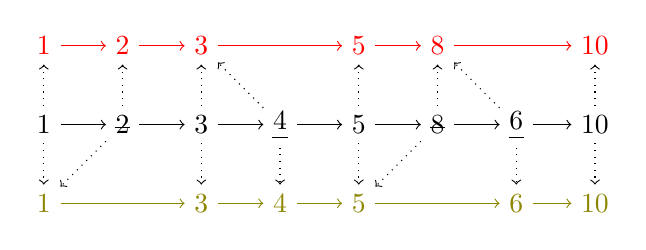
\begin{tikzpicture}
    \node (o1) {1};
    \node[right of=o1] (o2) {\st{2}};
    \node[right of=o2] (o3) {3};
    \node[right of=o3] (o4) {\ul{4}};
    \node[right of=o4] (o5) {5};
    \node[right of=o5] (o8) {\st{8}};
    \node[right of=o8] (o6) {\ul{6}};
    \node[right of=o6] (o10) {10};
    \draw[->] (o1) -- (o2);
    \draw[->] (o2) -- (o3);
    \draw[->] (o3) -- (o4);
    \draw[->] (o4) -- (o5);
    \draw[->] (o5) -- (o8);
    \draw[->] (o8) -- (o6);
    \draw[->] (o6) -- (o10);

    \node[red, above of=o1] (d1) {1};
    \node[red, above of=o2] (d2) {2};
    \node[red, above of=o3] (d3) {3};
    \node[red, above of=o5] (d5) {5};
    \node[red, above of=o8] (d8) {8};
    \node[red, above of=o10] (d10) {10};
    \draw[red, ->] (d1) -- (d2);
    \draw[red, ->] (d2) -- (d3);
    \draw[red, ->] (d3) -- (d5);
    \draw[red, ->] (d5) -- (d8);
    \draw[red, ->] (d8) -- (d10);
    \draw[dotted, ->] (o1) -- (d1);
    \draw[dotted, ->] (o2) -- (d2);
    \draw[dotted, ->] (o3) -- (d3);
    \draw[dotted, ->] (o4) -- (d3);
    \draw[dotted, ->] (o5) -- (d5);
    \draw[dotted, ->] (o8) -- (d8);
    \draw[dotted, ->] (o6) -- (d8);
    \draw[dotted, ->] (o10) -- (d10);

    \node[olive, below of=o1] (i1) {1};
    \node[olive, below of=o3] (i3) {3};
    \node[olive, below of=o4] (i4) {4};
    \node[olive, below of=o5] (i5) {5};
    \node[olive, below of=o6] (i6) {6};
    \node[olive, below of=o10] (i10) {10};
    \draw[olive, ->] (i1) -- (i3);
    \draw[olive, ->] (i3) -- (i4);
    \draw[olive, ->] (i4) -- (i5);
    \draw[olive, ->] (i5) -- (i6);
    \draw[olive, ->] (i6) -- (i10);
    \draw[dotted, ->] (o1) -- (i1);
    \draw[dotted, ->] (o2) -- (i1);
    \draw[dotted, ->] (o3) -- (i3);
    \draw[dotted, ->] (o4) -- (i4);
    \draw[dotted, ->] (o5) -- (i5);
    \draw[dotted, ->] (o8) -- (i5);
    \draw[dotted, ->] (o6) -- (i6);
    \draw[dotted, ->] (o10) -- (i10);
\end{tikzpicture}
\end{minipage}
\caption{Execution synchronization of a source and a destination program extracted from a difference tree without colors. For simplification, we show only one state for each line of code and consider that $c = \mathbf{false}$.}
\label{fig:oracle_sync_from_diff}
\end{figure}

Figure~\ref{fig:oracle_sync_from_diff} shows an example of such syncronization. Lines 2 and 4 are executed by only one program but we can resynchronize afterwards at the next spine node. As the control flow decision changes at line 5, we first let the original program execute line 8, then let the merged one execute line 6 and then resynchronize. At each step we advance in at least one of the programs, sometimes keeping the other stalled.

To express the interleaving between two programs, and compute the
colors of the expressions, we use the correlation oracle framework \cite{girka2017verifiable}.

Formally, a correlation oracle is defined as a program with states
that can be projected on either of the correlated programs.
Moreover, it carries extra information on the simultaneous executions of
both programs and compute (dynamically if needed) their synchronization points.
Intuitively, in our case it corresponds to the black execution line on Figure~\ref{fig:oracle_sync_from_diff}.
Its execution steps must correspond to executing steps in at least one of the correlated program.

The states of correlation oracles can be enriched with additional information on the co-execution. We use this flexibility for storing and computing our awareness colors on values.

\subsubsection{Specification of the colored difference oracle}

We now will present the specification of the correlation oracle we use for checking the absence of semantic ambiguities on merged programs written in our Rust subset.

The states of the correlation oracle follow the structure of the states of the language $\rtstate{\kappa}{v}{S}$ but all the individual components need to be adapted for interleaving:
First, each value stored in the oracle state (either $v$ or inside $S$) must exist in two versions (written $v^-$ and $v^+$) respectively corresponding to the values in execution of the original and the merged program. To track commit provenance, we also add a color $c$ stating which commits are aware of the $v^+$ value. Values in oracle states are triples $(v^-, v^+, c)$.
Then, the continuation $\kappa$ must encode the interleaving itself. Expressions inside it can be either deleted (\st{$instr$}$^c$), inserted (\ul{$instr$}$^c$), or preserved ($instr$), depending on whether they will be executed in the original program only, the merged program only or both.
Deleted and inserted expressions carry a color with them that indicate which commit is responsible for the splitted execution (or said differently, responsible for the change).

This definition makes it possible to define the required projections of an oracle state on its equivalent original (resp. merged) program state by removing all inserted (resp. deleted) instructions, and projecting values on their $v^-$ (resp. $v^+$) component.
For a store~$S$, we write $S^-$, $S^+$ and $S^c$ for the projections of values on the corresponding $v^-$, $v^+$ and color components.

To describe how interleaving is done, we give operational semantic reductions below (sorted by design ideas).
In all the rules, if an instruction in the continuation should be both
inserted and deleted according to the rules, it is simply
discarded. If it should be inserted (resp. deleted) twice with
different colors, we take the intersection (resp. union) of these
colors to follow the color composition rules of Section~\ref{sec:colors}.

\paragraph{Simply expanding instructions}
The rules from the underlying language can directly be reused for instructions
that only expand inside the continuation, because they do nothing apart from destructuring. In this case, we preserve
the deleted/inserted/preserved status and the color on the expansion.

For instance, this gives the following reduction rules (non-exhaustive list):
\newbox\boxoverarrow
\sbox\boxoverarrow{$\overrightarrow{stmt;}$}
\begin{align*}
\rtstate{\mathst{\{{\usebox\boxoverarrow}\ expr\}}^k \cdot \kappa}{(v^-, v^+, c)}{S} &\rightarrow \rtstate{\overrightarrow{\mathst{stmt}}^k\cdot \mathst{expr}^k \cdot \kappa}{((), v^+, c)}{S}\\
\rtstate{\mathul{x = e}^k \cdot \kappa}{(v^-, v^+, c)}{S} &\rightarrow \rtstate{\mathul{e}^k \cdot \mathul{x = \square}^k \cdot \kappa}{(v^-, (), \top)}{S}\\
\rtstate{e_1 \diamond e_2 \cdot \kappa}{(v^-, v^+, c)}{S} &\rightarrow \rtstate{e_1 \cdot \square \diamond e_2 \cdot \kappa}{((), (), \top)}{S}\\
\end{align*}

\paragraph{Instruction producing value}

For instructions that change the current value, we need to be careful
regarding the color of the result. There are three cases:

\begin{itemize}
  \item
    If the instruction is preserved, the output color is the
    intersection of the input colors.

  \item
    If the instruction is deleted, the color of the value is tainted
    by the color of the deletion. However, the input values do not
    taint the result.

  \item
    If the instruction is inserted, the output color is the
    intersection of the input colors and the color of the insertion.
\end{itemize}
\yrg{The justifications are missing.}

This leads to the following reduction rules:
\begin{align*}
\rtstate{x \cdot \kappa}{(v^-, v^+, c)}{S} &\rightarrow \rtstate{\kappa}{S(x)}{S}\\
\rtstate{\mathst{x}^k \cdot \kappa}{(v^-, v^+, c)}{S} &\rightarrow \rtstate{\kappa}{(S^-(x), v^+, c \cap k)}{S}\\
\rtstate{\mathul{x}^k \cdot \kappa}{(v^-, v^+, c)}{S} &\rightarrow \rtstate{\kappa}{(v^-, S^+(x), S^c(x) \cap k)}{S}\\
\rtstate{literal \cdot \kappa}{(v^-, v^+, c)}{S} &\rightarrow \rtstate{\kappa}{(literal, literal, \top)}{S}\\
\rtstate{\mathst{literal}^k \cdot \kappa}{(v^-, v^+, c)}{S} &\rightarrow \rtstate{\kappa}{(literal, v^+, c \cap k)}{S}\\
\rtstate{\mathul{literal}^k \cdot \kappa}{(v^-, v^+, c)}{S} &\rightarrow \rtstate{\kappa}{(v^-, literal, k)}{S}\\
\rtstate{\star \square \cdot \kappa}{(v^-, v^+, c)}{S} &\rightarrow \rtstate{\kappa}{(\star v^-, \star v^+, c)}{S}\\
\rtstate{\mathst{\star \square}^k \cdot \kappa}{(v^-, v^+, c)}{S} &\rightarrow \rtstate{\kappa}{(\star v^-, v^+, c \cap k)}{S}\\
\rtstate{\mathul{\star \square}^k \cdot \kappa}{(v^-, v^+, c)}{S} &\rightarrow \rtstate{\kappa}{(v^-, \star v^+, c \cap k)}{S}\\
\rtstate{(v_l^-, v_l^+, c_l) \diamond \square \cdot \kappa}{(v_r^-, v_r^+, c_r)}{S} &\rightarrow \rtstate{\kappa}{(v_l^- \diamond v_r^-, v_l^+ \diamond v_r^+, c_l \cap c_r)}{S}\\
\rtstate{\mathst{(v_l^-, v_l^+, c_l) \diamond \square}^k \cdot \kappa}{(v_r^-, v^+, c)}{S} &\rightarrow \rtstate{\kappa}{(v_l^- \diamond v_r^-, v^+, c \cap k)}{S}\\
\rtstate{\mathul{(v_l^-, v_l^+, c_l) \diamond \square}^k \cdot \kappa}{(v^-, v_r^+, c_r)}{S} &\rightarrow \rtstate{\kappa}{(v^-, v_l^+ \diamond v_r^+, c_l \cap c_r \cap k)}{S}\\
\end{align*}

\paragraph{Assignment instructions}
With the same ideas as instruction producing a value but this time inside the store, assignment instructions are treated as follows:
\begin{align*}
\rtstate{x = \square \cdot \kappa}{(v^-, v^+, c)}{S} &\rightarrow \rtstate{\kappa}{((), (), \top)}{S[x \leftarrow (v^-, v^+, c)]}\\
\rtstate{\mathst{x = \square}^k \cdot \kappa}{(v^-, v^+, c)}{S} &\rightarrow \rtstate{\kappa}{((), v^+, c \cap k)}{S[x \leftarrow (v^-, S^+(x), S^c(x) \cap k)]}\\
\rtstate{\mathul{x = \square}^k \cdot \kappa}{(v^-, v^+, c)}{S} &\rightarrow \rtstate{\kappa}{(v^-, (), k)}{S[x \leftarrow (S^-(x), v^+, c \cap k)]}\\
\end{align*}

\paragraph{Function calls} Function calls do not need any special treatment, they can be considered as instructions simply expanding the function body into the continuation. The arguments keep their colors at the call point.
However note that $\mathbb{G}(f)$ potentially contains code that is either deleted or inserted.
\newbox\boxargs
\sbox\boxargs{$\overrightarrow{(v_a^-, v_a^+, c_a)}$}
\begin{align*}
\rtstate{f(\usebox\boxargs) \cdot \kappa}{(v^-, v^+, c)}{S} &\rightarrow \rtstate{\mathbb{G}(f) \cdot \mathbf{eof} \cdot \kappa}{((), (), \top)}{\{\overrightarrow{a \leftarrow (v_a^-, v_a^+, c_a)}\} :: S}\\
\rtstate{\mathst{f(\usebox\boxargs)}^k \cdot \kappa}{(v^-, v^+, c)}{S} &\rightarrow \rtstate{\mathst{\mathbb{G}(f)}^k \cdot \mathst{\mathbf{eof}}^k \cdot \kappa}{((), v^+, c \cap k)}{\{\overrightarrow{a \leftarrow (v_a^-, v_a^+, c_a)}\} :: S}\\
\rtstate{\mathul{f(\usebox\boxargs)}^k \cdot \kappa}{(v^-, v^+, c)}{S} &\rightarrow \rtstate{\mathul{\mathbb{G}(f)}^k \cdot \mathul{\mathbf{eof}}^k \cdot \kappa}{(v^-, (), k)}{\{\overrightarrow{a \leftarrow (v_a^-, v_a^+, c_a)}\} :: S}\\
\end{align*}
To make a static analysis, this function inlining approach might become too expansive and it might be replaced by some intraprocedural analysis. This is left for future work.

\paragraph{Conditionals instructions} Conditional instruction are a bit harder to handle because they can split the execution between the correlated programs even when the branches themselves are totally in the spine. Indeed, both programs can show different value for the condition, and therefore take different paths. Also they could take the same value but only by chance and still be under the influence of some non-white color. In both case, we choose to split the execution and resynchronize only at the end of the branches.
\begin{align*}
\rtstate{\mathbf{if}\ \square\ b_{true}\ \mathbf{else}\ b_{false} \cdot  \kappa}{(\mathbf{true}, \mathbf{true}, \top)}{S} &\rightarrow \rtstate{b_{true} \cdot \kappa}{((), (), \top)}{S}\\
\rtstate{\mathbf{if}\ \square\ b_{true}\ \mathbf{else}\ b_{false} \cdot  \kappa}{(\mathbf{false}, \mathbf{false}, \top)}{S} &\rightarrow \rtstate{b_{false} \cdot \kappa}{((), (), \top)}{S}\\
\rtstate{\mathbf{if}\ \square\ b_{true}\ \mathbf{else}\ b_{false} \cdot \kappa}{(v^-, v^+, c)}{S} &\rightarrow \vrtstate{\mathst{\mathbf{if}\ \square\ b_{true}\ \mathbf{else}\ b_{false}}^c \cdot \mathul{\mathbf{if}\ \square\ b_{true}\ \mathbf{else}\ b_{false}}^c \cdot \kappa}{((), (), \top)}{S}\\
\end{align*}

To reduce a conditional that is deleted, we can simply take the matching branch, but if it is inserted, we need to also take into account the color of the condition. This leads to these rules:
\begin{align*}
\rtstate{\mathst{\mathbf{if}\ \square\ b_{true}\ \mathbf{else}\ b_{false}}^k \cdot  \kappa}{(\mathbf{true}, v^+, c)}{S} &\rightarrow \rtstate{\mathst{b_{true}}^k \cdot \kappa}{((), v^+, c)}{S}\\
\rtstate{\mathst{\mathbf{if}\ \square\ b_{true}\ \mathbf{else}\ b_{false}}^k \cdot  \kappa}{(\mathbf{false}, v^+, c)}{S} &\rightarrow \rtstate{\mathst{b_{false}}^k \cdot \kappa}{((), v^+, c)}{S}\\
\rtstate{\mathul{\mathbf{if}\ \square\ b_{true}\ \mathbf{else}\ b_{false}}^k \cdot \kappa}{(v^-, \mathbf{true}, c)}{S} &\rightarrow \rtstate{\mathul{b_{true}}^{k \cap c} \cdot \kappa}{(v^-, (), k)}{S}\\
\rtstate{\mathul{\mathbf{if}\ \square\ b_{true}\ \mathbf{else}\ b_{false}}^k \cdot \kappa}{(v^-, \mathbf{false}, c)}{S} &\rightarrow \rtstate{\mathul{b_{false}}^{k \cap c} \cdot \kappa}{(v^-, (), k)}{S}\\
\end{align*}

\paragraph{Control flow breaking instructions} For control flow breaking instructions (ie. \textbf{continue}, \textbf{break} and \textbf{return}), they are completely unchanged in their preserved mode. However, if they are either deleted or inserted, we cannot simply skip instructions as only one program does this. Therefore, we keep the skipped instructions but mark them as only executed by the opposite program. This leads to the following rules:
\begin{align*}
\rtstate{\mathst{\mathbf{continue}}^k \cdot \overrightarrow{\kappa_{\neg while}} \cdot \mathbf{while}\ e\ b \cdot \kappa}{(v^-, v^+, c)}{S} &\rightarrow \rtstate{\overrightarrow{\mathul{\kappa_{\neg while}}}^k \cdot \mathbf{while}\ e\ b \cdot \kappa}{((), v^+, c)}{S}\\
\rtstate{\mathul{\mathbf{continue}}^k \cdot \overrightarrow{\kappa_{\neg while}} \cdot \mathbf{while}\ e\ b \cdot \kappa}{(v^-, v^+, c)}{S} &\rightarrow \rtstate{\overrightarrow{\mathst{\kappa_{\neg while}}}^k \cdot \mathbf{while}\ e\ b \cdot \kappa}{(v^-, (), c)}{S}\\
\rtstate{\mathst{\mathbf{break}}^k \cdot \overrightarrow{\kappa_{\neg while}} \cdot \mathbf{while}\ e\ b \cdot \kappa}{(v^-, v^+, c)}{S} &\rightarrow \rtstate{\overrightarrow{\mathul{\kappa_{\neg while}}}^k \cdot \mathul{\mathbf{while}\ e\ b}^k \cdot \kappa}{((), v^+, c)}{S}\\
\rtstate{\mathul{\mathbf{break}}^k \cdot \overrightarrow{\kappa_{\neg while}} \cdot \mathbf{while}\ e\ b \cdot \kappa}{(v^-, v^+, c)}{S} &\rightarrow \rtstate{\overrightarrow{\mathst{\kappa_{\neg while}}}^k \cdot \mathst{\mathbf{while}\ e\ b}^k \cdot \kappa}{(v^-, (), c)}{S}\\
\rtstate{\mathst{\mathbf{return}\ \square}^k \cdot \overrightarrow{\kappa_{\neg eof}} \cdot \mathbf{eof} \cdot \kappa}{(v^-, v^+, c)}{S} &\rightarrow \rtstate{\overrightarrow{\mathul{\kappa_{\neg eof}}}^k \cdot \mathbf{eof} \cdot \kappa}{(v^-, v^+, c)}{S}\\
\rtstate{\mathul{\mathbf{return}\ \square}^k \cdot \overrightarrow{\kappa_{\neg eof}} \cdot \mathbf{eof} \cdot \kappa}{(v^-, v^+, c)}{S} &\rightarrow \rtstate{\overrightarrow{\mathst{\kappa_{\neg eof}}}^k \cdot \mathbf{eof} \cdot \kappa}{(v^-, v^+, c)}{S}\\
\end{align*}

The case where we are skipping code that was already executed by only one program is managed because we systematically skip instructions that are both deleted and inserted, and merge colors appropriately.

\paragraph{Enum related instructions} We could treat the enum values normally but we think it is a bad idea. Indeed when constructing an enum value, the color should normally be the intersection of all individual colors at the constructor call.
For a simple enum encoding pairs with constructor $P$, it means for instance that $P({\color{blue}v_1}, {\color{orange}v_2})$ would create a black value, while there is currently no ambiguity (yet).

To fix this problem, we introduce composite runtime colors. Runtime colors can be more complex than a single color. When the insertion value has an enum type, we store a color for the constructor and (potentially composite) colors for each of its arguments. It obeys the following rules:
\begin{align*}
\rtstate{C(\usebox\boxargs) \cdot \kappa}{(v^-, v^+, c)}{S} &\rightarrow \rtstate{\kappa}{(C(\overrightarrow{v_a^-}), C(\overrightarrow{v_a^+}), \top(\overrightarrow{c_a}))}{S}\\
\rtstate{\mathst{C(\usebox\boxargs)}^k \cdot \kappa}{(v^-, v^+, c)}{S} &\rightarrow \rtstate{\kappa}{(C(\overrightarrow{v_a^-}), v_+, c \cap k)}{S}\\
\rtstate{\mathul{C(\usebox\boxargs)}^k \cdot \kappa}{(v^-, v^+, c)}{S} &\rightarrow \rtstate{\kappa}{(v^-, C(\overrightarrow{v_a^+}), k(\overrightarrow{c_a \cap k}))}{S}\\
\end{align*}

Now when we encounter a \textbf{match}, that is destructuring an enum value, we apply the same strategy as with \textbf{if}s on the constructor and we recover the colors of the arguments in their destructured pattern variable. This corresponds to the rules below:
\newbox\boxmatch
\sbox\boxmatch{$\mathbf{match}\ \square\ \{ \overrightarrow{C(\overrightarrow{x_C,}) \Rightarrow e_C,} \}$}
\begin{align*}
\vrtstate{\usebox\boxmatch \cdot \kappa}{(D(\overrightarrow{v_D^-}), D(\overrightarrow{v_D^+}), \top(\overrightarrow{c_D}))}{S} &\rightarrow \rtstate{e_D \cdot \kappa}{((), (), \top)}{S\left[\overrightarrow{x_D \leftarrow (v_D^-, v_D^+, c_D)}\right]}\\
\vrtstate{\usebox\boxmatch \cdot \kappa}{(v^-, v^+, c)}{S} &\rightarrow \vrtstate{\mathst{\usebox\boxmatch}^c \cdot \mathul{\usebox\boxmatch}^c \cdot \kappa}{((), (), \top)}{S}\\
\vrtstate{\mathst{\usebox\boxmatch}^k \cdot \kappa}{(D(\overrightarrow{v_D^-}), v^+, c)}{S} &\rightarrow \rtstate{\mathst{e_D}^k \cdot \kappa}{((), v^+, c \cap k)}{S\left[\overrightarrow{x_D \leftarrow (v_D^-, S_{ins}(x_D), S_c(x_D))}\right]}\\
\vrtstate{\mathul{\usebox\boxmatch}^k \cdot \kappa}{(v^-, D(\overrightarrow{v_D^+}), c(\overrightarrow{c_D}))}{S} &\rightarrow \rtstate{\mathul{e_D}^{c \cap k} \cdot \kappa}{(v^-, (), k)}{S\left[\overrightarrow{x_D \leftarrow (S_{del}(x_D), v_D^+, c_D)}\right]}\\
\end{align*}

\paragraph{Continue after crash}
Executing some instructions (division by zero for instance) may crash one of the two correlated program but not the other. This is not a problem.

At a crash in the merged program we can end the analysis as no new ambiguities will be discovered. The crash point itself may or may not be declared ambiguous depending on the color of the instruction and the operands.

If the original program crashes however, we have to continue executing the merged program alone as only the effect of remaining deleted instructions is gone. To simulate that, we mark all the continuation as inserted with color white (following composition rules for already inserted instructions). The white color is chosen as we consider that fixing a crash will never break invariants of other commits. This is an assumption that might be questionned.

\paragraph{Interpreting a colored difference with this oracle formalism}
We can interpret non-conflicting self-contained differences as code for colored diffrence oracles.
Indeed, removed and inserted code directly map to removed and inserted expressions, and we only have to add a last reduction rule that splits the execution paths when needed.
$$\rtstate{\mathst{e_d}^k \rightarrow \mathul{e_i}^k \cdot \kappa}{(v^-, v^+, c)}{S} \rightarrow \rtstate{\mathst{e_d}^k \cdot \mathul{e_i}^k \cdot \kappa}{((), (), \top)}{S}$$
This was expected as we designed the merging algorithm and the way it propagates colors to match the semantic analysis given here.

\paragraph{Soundness of the reduction rules}
The soundness of the rules above is directly given by the interpretation of the color of a value, and therefore of an ambiguity. A value must have a given tint if and only if the corresponding commit is aware of it (or at least of all meaningful invariants linked to it) in the current program state.
All the unforseen interactions between concurrent commits might be source of bugs, but fortunately, all of them will generate black values. This is because by definition unforseen interaction occur when either two independantly modified values are combined or newly introduced code uses independantly modified value.

\paragraph{Ambiguity detection}

During the execution of the correlation oracle, ambiguities are
detected whenever the black color is found in the value. To avoid
stopping at the first ambiguity and be able to warn the user about
more than one problem at the same time, we can continue the execution
on a black value and locally replace it with white, signaling an
error to be manually resolved later. A merge is valid if it never
create such black value.

\subsection{Resolving conflicts and ambiguities}
The colored difference oracle reports a list of ambiguity points, that
must be resolved before having a valid merge. For our tool to be
practical, the manual ambiguity resolution should be easy and rather
quick as soon as the programmer who initiated the merge understand how
the commits interact at each ambiguity point. In this internship, I
propose resolution tactics that let a programmer alter the merge
candidate to progressively remove conflicts and ambiguities. As for
the semantic check, this part is purely theoretical as I had no time
for implementing it.

After each tactic application, our intended tool would recheck the
semantics for potential remaining ambiguities, until there is none
left. At the end of the process, we simply keep the projection on the
last merged candidate as the final merged program.

Currently we only have few resolution tactics but I think that they
are powerful enough for resolving all conflicts. However they trust
the programmer to ensure invariants and are quite low level so more
automated tactics could be added in future work.

\paragraph{Declare preserving semantic change}
%
Some changes are refactorings that do not modify the semantics, or are
bug fixes that do not change the intended semantics that rest of the
program rely on. The automatic ambiguity detection will be triggered
by these changes because it is unable to notice the constant implicit
semantic preservation. To mark these ambiguity as false positive, we
can use the \textit{preserving} tactic, that replace the color of a
change with constant semantic by white (the change can be the whole
commit or only some modifications). It represents the fact that being
aware or not of the modification is irrelevant as the user told us
that it does not change the meaning of the code, and it will
effectively remove the ambiguity.

\paragraph{Reviewed interaction block}
%
Sometimes, even if changes do not globally preserve semantics, after
manual check, their interaction does not cause any real problem. In
that case, the tactic \textit{reviewed} mark a block of code as still
keeping its intended semantic even if several modifications interact
inside. When the correlation oracle executes a reviewed block, the
color of the value is reset to white between each evaluation
step. Therefore, both final value, and variables assigned inside the
block are white after the block execution.
% \begin{align*}
% \rtstate{\mathbf{reviewed}\ e \cdot \kappa}{(v^-, v^+, c)}{S} &\rightarrow \rtstate{e \cdot \mathbf{eor} \cdot \kappa}{(v^-, v^+, \top^*)}{S}\\
% \rtstate{\mathbf{eor} \cdot \kappa}{(v^-, v^+, \top^*)}{S} &\rightarrow \rtstate{\kappa}{(v^-, v^+, \top)}{S}\\
% \end{align*}
% $\top^*$ is the color $\top$ but for any program step, no matter the rule used (except $\mathbf{eor}$), the output state color stays $\top^*$.

\paragraph{Revert a change}
%
Some changes will not compose well and with global knowledge reverting
them is simply the thing to do. The \textit{revert} tactic takes a
position in the difference tree and either removes inserted code,
restores deleted code or both.

\paragraph{Introduce a new change}
%
Similarly, in order to do some manual adjustments it could be
necessary to use a tactic that manually adds a change somewhere after
the automatic syntactic merge. As it is done in order to restore some
semantics after all the modifications are known, we can directly mark
this new change as \textit{reviewed}.

\paragraph{Resolve syntactic conflicts}
%
We can also use this tactic system to resolve the syntactic conflicts
that prevent the colored difference oracle to run. To do so, we add
tactics that resolve conflicts, locally reverting one change to keep
only the other, fix the insertion order, or force a meta-variable
replacement.

\section{Related work}
\label{sec:related-work}
Trying to give good representation for program differences is a well studied subject. Historically, we use algorithms solving longest common subsequence \cite{wagner1974string} and compare files line by line (the well known diff Unix tool \cite{hunt1976algorithm} use this approach).
Subsequent works studied how to get more structured differences by using trees instead of lines, reducing to the tree edit distance problem \cite{bille2005survey} instead.
Some more recent works (like the GumTree algorithm \cite{falleri2014fine}) wanted to take into account the fact that code can be moved around by programmers. A later refinement showed that even copy-paste-modify interactions can be captured \cite{higo2017generating}.

But these untyped differences can, when applied, produce programs that do not necessarily follow the syntax of the programming language. Therefore, datatype (or syntax) driven differences were introduced. The first approach considered actions on a stack of typed sub-trees \cite{lempsink2009type}. This seems hard to work with in a merging context, but a later refinement \cite{vassena2016generic} gave a merging algorithm nonetheless but failed to give typing guarantee in the merged output. A concurrent vision lead to representing the structured changes as tree themselves \cite{miraldo2017type} with spine, sequence edit scripts and change nodes. Later refinements introduced the notion of meta-variables for dealing with moved code \cite{miraldo2019efficient}. These two last papers highly inspired our difference algorithm. However, the proposed merge algorithm in \cite{miraldo2019efficient} only works if changes are fully disjoint and needed to be heavily completed to meet our goals.

Completely different studies focus on how to semantically characterize changes instead of caring about their syntax. To do so, they introduce logical frameworks that interleave the two considered programs and enable reasoning about states facing each other. Relational Hoare logic \cite{benton2004simple} is one of such framework. As it cannot prove anything on programs that do not crash at the same time and we thought that bug fixes are important changes, we preferred to use the correlation oracle formalism \cite{girka2017verifiable} developed later that address this issue. The difference language proposed along correlation oracles require manual difference labelling (and proving) and would have required a quadratic human work in the number of considered changes for implementing a merge algorithm. Therefore we chose to use the formalism without its proposed difference system.

Prior work \cite{girka2015mechanically} already used the general idea of letting a difference syntax tree drive the semantic interleaving, but did not try any kind of merging on its language specific difference language.

Besides, the awareness color mechanism that we use in the analysis can be compared to a form of provenance analysis \cite{cheney2007provenance}. 

\yrg{You should add a section about the implementation, or at the very least,
a reference to the tool's git repository with a clear description of what it
does.}\gb{I talk about it in Section~\ref{sec:codegen} now, I really have no space for a real implementation section}

\begin{appendices}
\renewcommand{\refname}{\section{References}}
\bibliographystyle{plain}
\bibliography{references}

\section{Specification of difference application}
\label{app:diff_application_spec}

The implied function of a difference tree is formally defined as follows: let us suppose that we have $\Gamma$ a function from meta-variables (occurring in the difference tree) to syntax trees. In practice, $\Gamma$ is constrained enough to be uniquely inferred by the algorithm given in Section~\ref{sec:diff_application}.

We denote by $h :: t$ a sequence containing at least one element, and by $[]$ the empty sequence.

A judgment $\Gamma \vdash t(d) = i$ means that under meta-variable replacements $\Gamma$, the difference tree $t$ applied to $d$ is well defined and returns $i$. The judgment $\Gamma \vdash c(d)$ means that the change $c$ is compatible with the original tree $d$ under meta-variable replacements $\Gamma$.

For any judgment, if we denote $\overrightarrow{x} = (x_0, \ldots, x_n)$, then $\overrightarrow{\Gamma \vdash x(y) = z}$ corresponds to $\forall k \in [\![ 0, n ]\!], \Gamma \vdash x_k(y_k) = z_k$ (and similarly for any judgment).
\gb{I really think that vector of judgments are more readable than $\forall (t^k, d_t^k) \in \overrightarrow{(t, d_t)}, \Gamma \vdash t^k(d_t^k) = i_t^k$ everywhere. Maybe I didn't understood the comment...}

Then, apply the following syntax-driven rules:

\begin{prooftree}
 \AxiomC{}
 \RightLabel{\textsc{Id}}
 \UnaryInfC{$\Gamma \vdash \id(t) = t$}
\end{prooftree}

\begin{prooftree}
 \AxiomC{$\Gamma \vdash d(t)$}
 \RightLabel{\textsc{Change}}
 \UnaryInfC{$\Gamma \vdash (\change{d}{i})(t) = \Gamma(i)$}
\end{prooftree}

\begin{prooftree}
 \AxiomC{$\overrightarrow{\Gamma \vdash t(d_t) = i_t}$}
 \AxiomC{$\overrightarrow{\Gamma \vdash s(d_s) = i_s}$}
 \RightLabel{\textsc{Spine}}
 \BinaryInfC{$\Gamma \vdash S(\overrightarrow{t},\overrightarrow{s})(S(\overrightarrow{d_t},\overrightarrow{d_s})) = S(\overrightarrow{i_t}, \overrightarrow{i_s})$}
\end{prooftree}

\begin{prooftree}
 \AxiomC{$\Gamma \vdash t(d) = i$}
 \AxiomC{$\Gamma \vdash r(d_r) = i_r$}
 \RightLabel{\textsc{SeqZip}}
 \BinaryInfC{$\Gamma \vdash (t::r)(d::d_r) = i::i_r$}
\end{prooftree}

\begin{prooftree}
 \AxiomC{$\Gamma \vdash c(d)$}
 \AxiomC{$\Gamma \vdash r(d_r) = i_r$}
 \RightLabel{\textsc{SeqDel}}
 \BinaryInfC{$\Gamma \vdash (\mathst{c}::r)(d::d_r) = i_r$}
\end{prooftree}

\begin{prooftree}
 \AxiomC{$\Gamma \vdash r(d_r) = i_r$}
 \RightLabel{\textsc{SeqIns}}
 \UnaryInfC{$\Gamma \vdash (\mathul{c}::r)(d_r) = \Gamma(c) :: i_r$}
\end{prooftree}

\begin{prooftree}
 \AxiomC{}
 \RightLabel{\textsc{SeqEmpty}}
 \UnaryInfC{$\Gamma \vdash []([]) = []$}
\end{prooftree}

\begin{prooftree}
 \AxiomC{$\Gamma(\alpha) = d$}
 \RightLabel{\textsc{DelMv}}
 \UnaryInfC{$\Gamma \vdash \alpha(d)$}
\end{prooftree}

\begin{prooftree}
 \AxiomC{$\overrightarrow{\Gamma \vdash c_t(d_t)}$}
 \AxiomC{$\overrightarrow{\Gamma \vdash c_s(d_s)}$}
 \RightLabel{\textsc{DelSyn}}
 \BinaryInfC{$\Gamma \vdash S(\overrightarrow{c_t}, \overrightarrow{c_s})(S(\overrightarrow{d_t}, \overrightarrow{d_s}))$}
\end{prooftree}

\section{Example of code generator usage}
\label{app:codegen}

\begin{lstlisting}[label=lst:codegen, caption={Usage example of the code generator for creating the hash-tagged family variant}]
syn_codegen! {
    pub mod hash {
        use crate::family_traits::Convert;
        use crate::hash_tree::{HashTagged, TreeHasher};

        #[derive(Hash, Eq, PartialEq)]
        extend_family! {
            Expr as HashTagged<Expr>,
            Vec<Stmt> as Vec<HashTagged<Stmt>>,
            Vec<Item> as Vec<HashTagged<Item>>,
            [...] // other type replacements
        }

        family_impl!(Convert<syn, self> for TreeHasher);
    }

    [...] // other family variants
}
\end{lstlisting}

This shows how the code genarator can be used a hash-tagged family variant of the syn syntax trees. The macro call \verb$extend_family!$, is replaced by a copy of the syn type tree where some types are enriched.
For instance, all vectors of \verb$Stmt$ are replaced by vectors of \verb$HashTagged<Stmt>$. This generates a copy of the 180+ types of the syn family. Then \verb$family_impl!$ implement a trait \verb$Convert$ for the type \verb$TreeHasher$ on all pairs of enums and struct from the family variants \verb$syn$ (the default one) and \verb$self$ the one inside the current module. For instance, trait \verb$Convert<syn::Expr, hash::Expr>$ is implemented for \verb$TreeHasher$ with a simple structural recursive conversion. However, this implementation relies on non provided implementations like \verb$Convert<syn::Expr, HashTagged<hash::Expr>>$, that must be manually given because the code generator cannot guess how to convert into the type replacement.

\section{Specification of the difference merging algorithm}
\label{app:syntactic_merge_spec}

The difference merging algorithm is defined modulo two replacement
functions $\Gamma$ and $\Delta$ from meta-variables to respectively
insertion and deletion trees, that are heavily constrained and in
practice inferred during the merge as seen in Section~\ref{sec:syntactic_merge_algo}.

The specification is based on several judgments:
\begin{itemize}
 \item The main one $\Gamma, \Delta \vdash t_l \merge t_r = t$ states that under meta-variable replacements $\Gamma$ and $\Delta$ the syntactic merge of $t_l$ and $t_r$ is well defined and has the output $t$. This declines for difference trees and sequences. 
 \item $\Gamma \vdash i \subset d = d'$ means that under replacements $\Gamma$, $i$ can be inlined into $d$ forming the deletion tree $d'$. Its negative counterpart is $\Gamma \vdash i \not\subset d$. 
 \item $\Gamma \vdash d$ means that if nothing is inlined inside, $d$ is compatible with replacements in $\Gamma$.
 \item $\Delta \vdash d_l \wedge d_r = d$, means that under replacements $\Delta$, $d_l$ and $d_r$ can be merged into a deletion tree $d$ representing the intersection of the trees accepted by $d_l$ and $d_r$.
 \item $\Gamma \vdash i_l \vee i_r = i$, means that under replacements $\Gamma$, $i_l$ and $i_r$ can be merged into insertion tree $i$.
\end{itemize}
Besides, this section follows the same notations as Appendix~\ref{app:diff_application_spec}.

\yrg{This will take you some time but it is mandatory to:
(i) enumerate and explain each judgment and how it is read ;
(ii) give some informal explanation for each rule.}\gb{(i) done; (ii) probably too long for the time I have left given the fact that it is ``only'' an Appendix now that ``may or may not be read''}

\begin{prooftree}
 \AxiomC{$\Gamma, \Delta \vdash t_r \merge t_l = t$}
 \RightLabel{\textsc{Symmetry}}
 \UnaryInfC{$\Gamma, \Delta \vdash t_l \merge t_r = t$}
\end{prooftree}

\paragraph{Merge spine nodes}
\begin{prooftree}
 \AxiomC{}
 \RightLabel{\textsc{Id}}
 \UnaryInfC{$\Gamma, \Delta \vdash t \merge \id = \Delta(\Gamma(t))$}
\end{prooftree}

\begin{prooftree}
 \AxiomC{$\overrightarrow{\Gamma, \Delta \vdash t_l \merge t_r = t}$}
 \AxiomC{$\overrightarrow{\Gamma, \Delta \vdash s_l \merge s_r = s}$}
 \RightLabel{\textsc{Spine}}
 \BinaryInfC{$\Gamma, \Delta \vdash S(\overrightarrow{t_l}, \overrightarrow{s_l}) \merge S(\overrightarrow{t_r}, \overrightarrow{s_r}) = S(\overrightarrow{t}, \overrightarrow{s})$}
\end{prooftree}

\newbox\boxspinenode
\sbox\boxspinenode{$S(\overrightarrow{t}, \overrightarrow{s})$}
\begin{prooftree}
 \AxiomC{$\Gamma, \Delta \vdash (\change{\usebox\boxspinenode}{\usebox\boxspinenode}) \merge (\change{d_r}{i_r}) = c$}
 \RightLabel{\textsc{Unwind}}
 \UnaryInfC{$\Gamma, \Delta \vdash \usebox\boxspinenode \merge (\change{d_r}{i_r}) = c$}
\end{prooftree}

\begin{prooftree}
 \AxiomC{$\Gamma \vdash i_l \not\subset d_r$}
 \AxiomC{$\Gamma \vdash i_r \not\subset d_l$}
 \AxiomC{$\Gamma \vdash d_l$}
 \AxiomC{$\Gamma \vdash d_r$}
 \RightLabel{\textsc{ChNoInl}}
 \QuaternaryInfC{$\Gamma, \Delta \vdash (\change{d_l}{i_l}) \merge (\change{d_r}{i_r}) = (\change{d_l \wedge d_r}{i_l \vee i_r})$}
\end{prooftree}

\begin{prooftree}
 \AxiomC{$\Gamma \vdash i_l \subset d_r = d'$}
 \AxiomC{$\Gamma \vdash i_r \not\subset d_l$}
 \AxiomC{$\Gamma \vdash d_l$}
 \RightLabel{\textsc{ChOneInl}}
 \TrinaryInfC{$\Gamma, \Delta \vdash (\change{d_l}{i_l}) \merge (\change{d_r}{i_r}) = (\change{d' \wedge d_l}{\Gamma(i_r)})$}
\end{prooftree}

\begin{prooftree}
 \AxiomC{$\Gamma \vdash i_l \subset d_r$}
 \AxiomC{$\Gamma \vdash i_r \subset d_l$}
 \AxiomC{$\Gamma \vdash d_l$}
 \AxiomC{$\Gamma \vdash d_r$}
 \RightLabel{\textsc{ChBothInl}}
 \QuaternaryInfC{$\Gamma, \Delta \vdash (\change{d_l}{i_l}) \merge (\change{d_r}{i_r}) = (\change{d_l \wedge d_r}{i_l \vee i_r})$}
\end{prooftree}

\paragraph{Merge sequence edit scripts (except insertions)}
\begin{prooftree}
 \AxiomC{}
 \RightLabel{\textsc{EmptySeq}}
 \UnaryInfC{$\Gamma, \Delta \vdash [] \merge [] = []$}
\end{prooftree}

\begin{prooftree}
 \AxiomC{$\Gamma, \Delta \vdash t_l \merge t_r = t$}
 \AxiomC{$\Gamma, \Delta \vdash r_l \merge r_r = r$}
 \RightLabel{\textsc{BothZip}}
 \BinaryInfC{$\Gamma, \Delta \vdash (t_l :: r_l) \merge (t_r :: r_r) = t :: r$}
\end{prooftree}

\begin{prooftree}
 \AxiomC{$\Gamma \vdash d_l$}
 \AxiomC{$\Gamma \vdash d_r$}
 \AxiomC{$\Gamma, \Delta \vdash r_l \merge r_r = r$}
 \RightLabel{\textsc{BothDel}}
 \TrinaryInfC{$\Gamma, \Delta \vdash (\mathst{d_l} :: r_l) \merge (\mathst{d_r} :: r_r) = \mathst{d_l \wedge d_r} :: r$}
\end{prooftree}

\begin{prooftree}
 \AxiomC{$t_r = \change{d_r}{i_r}$}
 \AxiomC{$\Gamma \vdash i_r \subset d_l = d'$}
 \AxiomC{$\Gamma \vdash d_r$}
 \AxiomC{$\Gamma, \Delta \vdash r_l \merge r_r = r$}
 \RightLabel{\textsc{DelZipInline}}
 \QuaternaryInfC{$\Gamma, \Delta \vdash (\mathst{d_l} :: r_l) \merge (t_r :: r_r) = \mathst{d' \wedge d_r} :: r$}
\end{prooftree}

\begin{prooftree}
 \AxiomC{$t_r = \change{d_r}{i_r}$}
 \AxiomC{$\Gamma \vdash i_r \not\subset d_l$}
 \AxiomC{$\Gamma \vdash d_l$}
 \AxiomC{$\Gamma \vdash d_r$}
 \AxiomC{$\Gamma, \Delta \vdash r_l \merge r_r = r$}
 \RightLabel{\textsc{DelZipConflict}}
 \QuinaryInfC{$\Gamma, \Delta \vdash (\mathst{d_l} :: r_l) \merge (t_r :: r_r) = \DelConflict(d_l \wedge d_r, \Gamma(i_r)) :: r$}
\end{prooftree}

\begin{prooftree}
 \AxiomC{$\Gamma \vdash i_l \not\subset d_r$}
 \AxiomC{$\Gamma \vdash i_r \not\subset d_l$}
 \AxiomC{$\Gamma \vdash d_l$}
 \AxiomC{$\Gamma \vdash d_r$}
 \AxiomC{$\Gamma, \Delta \vdash r_l \merge r_r = r$}
 \RightLabel{\textsc{DelConflNoInl}}
 \QuinaryInfC{$\Gamma, \Delta \vdash (\DelConflict(d_l, i_l) :: r_l) \merge (\DelConflict(d_r, i_r) :: r_r) = \DelConflict(d_l \wedge d_r, i_l \vee i_r) :: r$}
\end{prooftree}

\begin{prooftree}
 \AxiomC{$\Gamma \vdash i_l \subset d_r = d'_r$}
 \AxiomC{$\Gamma \vdash i_r \not\subset d_l$}
 \AxiomC{$\Gamma \vdash d_l$}
 \AxiomC{$\Gamma, \Delta \vdash r_l \merge r_r = r$}
 \RightLabel{\textsc{DelConflOneInl}}
 \QuaternaryInfC{$\Gamma, \Delta \vdash (\DelConflict(d_l, i_l) :: r_l) \merge (\DelConflict(d_r, i_r) :: r_r) = \DelConflict(d_l \wedge d'_r, \Gamma(i_r)) :: r$}
\end{prooftree}

\begin{prooftree}
 \AxiomC{$\Gamma \vdash i_l \subset d_r = d'_r$}
 \AxiomC{$\Gamma \vdash i_r \subset d_l = d'_l$}
 \AxiomC{$\Gamma, \Delta \vdash r_l \merge r_r = r$}
 \RightLabel{\textsc{DelConflBothInl}}
 \TrinaryInfC{$\Gamma, \Delta \vdash (\DelConflict(d_l, i_l) :: r_l) \merge (\DelConflict(d_r, i_r) :: r_r) = \mathst{d'_l \wedge d'_r} :: r$}
\end{prooftree}

\begin{prooftree}
 \AxiomC{$t_r = \change{d_r}{i_r}$}
 \AxiomC{$\Gamma, \Delta \vdash (\DelConflict(d_l, i_l) :: r_l) \merge (\DelConflict(d_r, i_r) :: r_r) = r$}
 \RightLabel{\textsc{DelConflZip}}
 \BinaryInfC{$\Gamma, \Delta \vdash (\DelConflict(d_l, i_l) :: r_l) \merge (t_r :: r_r) = r$}
\end{prooftree}

\begin{prooftree}
 \AxiomC{$\Gamma \vdash i_l \not\subset d_r$}
 \AxiomC{$\Gamma \vdash d_r$}
 \AxiomC{$\Gamma \vdash d_l$}
 \AxiomC{$\Gamma, \Delta \vdash r_l \merge r_r = r$}
 \RightLabel{\textsc{DelConflDelNoInl}}
 \QuaternaryInfC{$\Gamma, \Delta \vdash (\DelConflict(d_l, i_l) :: r_l) \merge (\mathst{d_r} :: r_r) = \DelConflict(d_l \wedge d_r, \Gamma(i_l)) :: r$}
\end{prooftree}

\begin{prooftree}
 \AxiomC{$\Gamma \vdash i_l \subset d_r = d'_r$}
 \AxiomC{$\Gamma \vdash d_l$}
 \AxiomC{$\Gamma, \Delta \vdash r_l \merge r_r = r$}
 \RightLabel{\textsc{DelConflDelInl}}
 \TrinaryInfC{$\Gamma, \Delta \vdash (\DelConflict(d_l, i_l) :: r_l) \merge (\mathst{d_r} :: r_r) = \mathst{d_l \wedge d'_r} :: r$}
\end{prooftree}

\paragraph{Merge insertions in sequence edit scripts}

\begin{prooftree}
 \AxiomC{$s_r \neq \mathul{\cdot}$}
 \AxiomC{$s_r \neq \OrdConflict(\cdot)$}
 \AxiomC{$\Gamma, \Delta \vdash r_l \merge (s_r :: r_r) = r$}
 \RightLabel{\textsc{InsBefore}}
 \TrinaryInfC{$\Gamma, \Delta \vdash (\mathul{i_l} :: r_l) \merge (s_r :: r_r) = \mathul{\Gamma(i_l)} :: r$}
\end{prooftree}

\begin{prooftree}
 \AxiomC{$\Gamma, \Delta \vdash r_l \merge [] = r$}
 \RightLabel{\textsc{InsEnd}}
 \UnaryInfC{$\Gamma, \Delta \vdash (\mathul{i_l} :: r_l) \merge [] = \mathul{\Gamma(i_l)} :: r$}
\end{prooftree}

\begin{prooftree}
 \AxiomC{$\Gamma(i_l) = \Gamma(i_r) = i$}
 \AxiomC{$\Gamma, \Delta \vdash r_l \merge r_r = r$}
 \RightLabel{\textsc{InsSame}}
 \BinaryInfC{$\Gamma, \Delta \vdash (\mathul{i_l} :: r_l) \merge (\mathul{i_r} :: r_r) = \mathul{i} :: r$}
\end{prooftree}

\begin{prooftree}
 \AxiomC{$\Gamma, \Delta \vdash r_l \merge r_r = r$}
 \RightLabel{\textsc{OrdConfl}}
 \UnaryInfC{$\Gamma, \Delta \vdash (\mathul{i_l} :: r_l) \merge (\mathul{i_r} :: r_r) = \OrdConflict([\Gamma(i_l), \Gamma(i_r)]) :: r$}
\end{prooftree}

\begin{prooftree}
 \AxiomC{$s_r \neq \mathul{\cdot}$}
 \AxiomC{$s_r \neq \OrdConflict(\cdot)$}
 \AxiomC{$\Gamma, \Delta \vdash r_l \merge (s_r :: r_r) = r$}
 \RightLabel{\textsc{OrdConflBefore}}
 \TrinaryInfC{$\Gamma, \Delta \vdash (\OrdConflict(i_l) :: r_l) \merge (s_r :: r_r) = \OrdConflict(\Gamma(i_l)) :: r$}
\end{prooftree}

\begin{prooftree}
 \AxiomC{$\Gamma, \Delta \vdash r_l \merge r_r = r$}
 \RightLabel{\textsc{OrdConflPush}}
 \UnaryInfC{$\Gamma, \Delta \vdash (\mathul{i_l} :: r_l) \merge (\OrdConflict(i_r) :: r_r) = \OrdConflict(\Gamma(i_l) :: \Gamma(i_r)) :: r$}
\end{prooftree}

\begin{prooftree}
 \AxiomC{$\Gamma, \Delta \vdash r_l \merge r_r = r$}
 \RightLabel{\textsc{OrdConflMerge}}
 \UnaryInfC{$\Gamma, \Delta \vdash (\OrdConflict(i_l) :: r_l) \merge (\OrdConflict(i_r) :: r_r) = \OrdConflict(\Gamma(i_l) \mathbin{@} \Gamma(i_r)) :: r$}
\end{prooftree}
With $\mathbin{@}$ being list concatenation.

\paragraph{Inclusion of insertion inside a deletion}\phantom{ }

\noindent
\begin{minipage}{.49\textwidth}
\begin{prooftree}
 \AxiomC{$\overrightarrow{\Gamma \vdash i \subset d = d'}$}
 \RightLabel{\textsc{SynIncl}}
 \UnaryInfC{$\Gamma \vdash S(\overrightarrow{i}) \subset S^c(\overrightarrow{d}) = S^c(\overrightarrow{d'})$}
\end{prooftree}

\begin{prooftree}
 \AxiomC{$\Gamma(\alpha)^{c \cup c'} = \Gamma(i)^c$}
 \RightLabel{\textsc{MvIncl}}
 \UnaryInfC{$\Gamma \vdash i \subset \alpha = \alpha$}
\end{prooftree}
\end{minipage}\hfill
\begin{minipage}{.49\textwidth}
\begin{prooftree}
 \AxiomC{$d \neq \alpha$}
 \AxiomC{$d \neq S(\cdot)$}
 \RightLabel{\textsc{SynNotIncl}}
 \BinaryInfC{$\Gamma \vdash S(\cdot) \not\subset d$}
\end{prooftree}

\begin{prooftree}
 \AxiomC{$d \neq \alpha$}
 \AxiomC{$i \neq S(\cdot)$}
 \RightLabel{\textsc{InsNotIncl}}
 \BinaryInfC{$\Gamma \vdash i \not\subset d$}
\end{prooftree}
\end{minipage}

\begin{prooftree}
 \AxiomC{$\Gamma(\alpha) = \top$}
 \RightLabel{\textsc{MvConfl}}
 \UnaryInfC{$\Gamma \vdash i \subset \alpha = \MvConflict(\alpha, \alpha, i)$}
\end{prooftree}

\begin{prooftree}
 \AxiomC{$\Gamma(\alpha) = \top$}
 \RightLabel{\textsc{MvConflPush}}
 \UnaryInfC{$\Gamma \vdash i \subset \MvConflict(\alpha, d, i') = \MvConflict(\alpha, d, i \vee i')$}
\end{prooftree}

\paragraph{Coherence with $\Gamma$ of kept deletion trees}\phantom{ }

\noindent\begin{minipage}{0.49\textwidth}
\begin{prooftree}
 \AxiomC{$\overrightarrow{\Gamma \vdash d}$}
 \RightLabel{\textsc{KeptSyn}}
 \UnaryInfC{$\Gamma \vdash S(\overrightarrow{d})$}
\end{prooftree}
\end{minipage}\hfill
\begin{minipage}{0.49\textwidth}
\begin{prooftree}
 \AxiomC{$\Gamma(\alpha) = \top$}
 \AxiomC{$\Gamma \vdash d$}
 \RightLabel{\textsc{KeptMvConfl}}
 \BinaryInfC{$\Gamma \vdash \MvConflict(\alpha, d, i)$}
\end{prooftree}
\end{minipage}

\begin{prooftree}
 \AxiomC{$\Gamma(\alpha) \in \{ \oplus(\Delta(\alpha)), \top \}$}
 \RightLabel{\textsc{KeptMv}}
 \UnaryInfC{$\Gamma \vdash \alpha$}
\end{prooftree}

Where $\oplus$ is a function transposing a deletion tree to an insertion tree by passing through each meta-variable conflict so that $\oplus(\MvConflict(\alpha, d, i)) = \oplus(d)$. It also replace every color by white.

\paragraph{Deletion alignment}\phantom{ }

\noindent\begin{minipage}{0.49\textwidth}
\begin{prooftree}
 \AxiomC{$\overrightarrow{\Delta \vdash d_l \wedge d_r = d}$}
 \RightLabel{\textsc{SameSyn}}
 \UnaryInfC{$\Delta \vdash S^{c_l}(\overrightarrow{d_l}) \wedge S^{c_r}(\overrightarrow{d_r}) = S^{c_l \cup c_r}(\overrightarrow{d})$}
\end{prooftree}

\begin{prooftree}
 \AxiomC{}
 \RightLabel{\textsc{SameMv}}
 \UnaryInfC{$\Delta \vdash \alpha^{c_l} \wedge \alpha^{c_r} = \Delta(\alpha)^{c_l \cup c_r}$}
\end{prooftree}
\end{minipage}\hfill
\begin{minipage}{0.49\textwidth}
\begin{prooftree}
 \AxiomC{$\Delta \vdash \Delta(\alpha) \wedge d_r = \Delta(\alpha)$}
 \RightLabel{\textsc{MvLeft}}
 \UnaryInfC{$\Delta \vdash \alpha^{c_l} \wedge d_r^{c_r} = \Delta(\alpha)^{c_l \cup c_r}$}
\end{prooftree}

\begin{prooftree}
 \AxiomC{$\Delta \vdash \Delta(\alpha) \wedge d_l = \Delta(\alpha)$}
 \RightLabel{\textsc{MvRight}}
 \UnaryInfC{$\Delta \vdash d_l^{c_l} \wedge \alpha^{c_r} = \Delta(\alpha)^{c_l \cup c_r}$}
\end{prooftree}
\end{minipage}

\begin{prooftree}
 \AxiomC{$\Delta \vdash d_l \wedge d_r = d$}
 \RightLabel{\textsc{MvConflLeft}}
 \UnaryInfC{$\Delta \vdash \MvConflict(\alpha, d_l^{c_l}, i) \wedge d_r^{c_r} = \MvConflict(\alpha, d^{c_l \cup c_r}, \Gamma(i))$}
\end{prooftree}

\begin{prooftree}
 \AxiomC{$\Delta \vdash d_l \wedge d_r = d$}
 \RightLabel{\textsc{MvConflRight}}
 \UnaryInfC{$\Delta \vdash d_l^{c_l} \wedge \MvConflict(\alpha, d_r^{c_r}, i) = \MvConflict(\alpha, d^{c_l \cup c_r}, \Gamma(i))$}
\end{prooftree}

\paragraph{Insertion alignment}

\begin{prooftree}
 \AxiomC{$\Gamma(i_l)^{c_l} = \Gamma(i_r)^{c_r} = i$}
 \RightLabel{\textsc{SameIns}}
 \UnaryInfC{$\Gamma \vdash i_l \vee i_r = i^{c_l \cup c_r}$}
\end{prooftree}

\begin{prooftree}
 \AxiomC{$\overrightarrow{\Gamma \vdash i_l \vee i_r = i}$}
 \RightLabel{\textsc{InsSyn}}
 \UnaryInfC{$\Gamma \vdash S^{c_l}(\overrightarrow{i_l}) \vee S^{c_r}(\overrightarrow{i_r}) = S^{c_l \cup c_r}(\overrightarrow{i})$}
\end{prooftree}

\begin{prooftree}
 \AxiomC{}
 \RightLabel{\textsc{InsConfl}}
 \UnaryInfC{$\Gamma \vdash i_l \vee i_r = \InsConflict(\Gamma(i_l), \Gamma(i_r))$}
\end{prooftree}

\end{appendices}
\end{document}
